\documentclass[master=eaict]{kulemt}
\setup{% Remove the "%" on the next line when using UTF-8 character encoding
  inputenc=utf8,
  title={Evaluating a Binocular dual-SSVEP Paradigm in Virtual Reality},
  author={Alken Rrokaj\and Fatjon Barçi},
  promotor={Prof.\,dr. Toon van Waterschoot},
  assessor={Prof.\,dr. Marc Van Hulle},
  assistant={Liuyin Yang}}

% \RequirePackage{pkgcheck}

% Choose the main text font (e.g., Latin Modern)
\setup{font=lm}

\usepackage[pdfusetitle,colorlinks=true,urlcolor=blue,citecolor=blue,linkcolor=blue,plainpages=false]{hyperref}


% Load necessary packages and styles
\usepackage{tabularx}
\usepackage{amssymb} % for \varnothing
\usepackage{multicol}
\usepackage{pdflscape} 
\usepackage{subcaption}
\usepackage{makecell}

\usepackage{eso-pic} % for cover fig
\AddToShipoutPictureBG*{%
  \AtPageLowerLeft{%
    \hspace{\dimexpr(\paperwidth-17cm)/2\relax}%
    \raisebox{21cm}{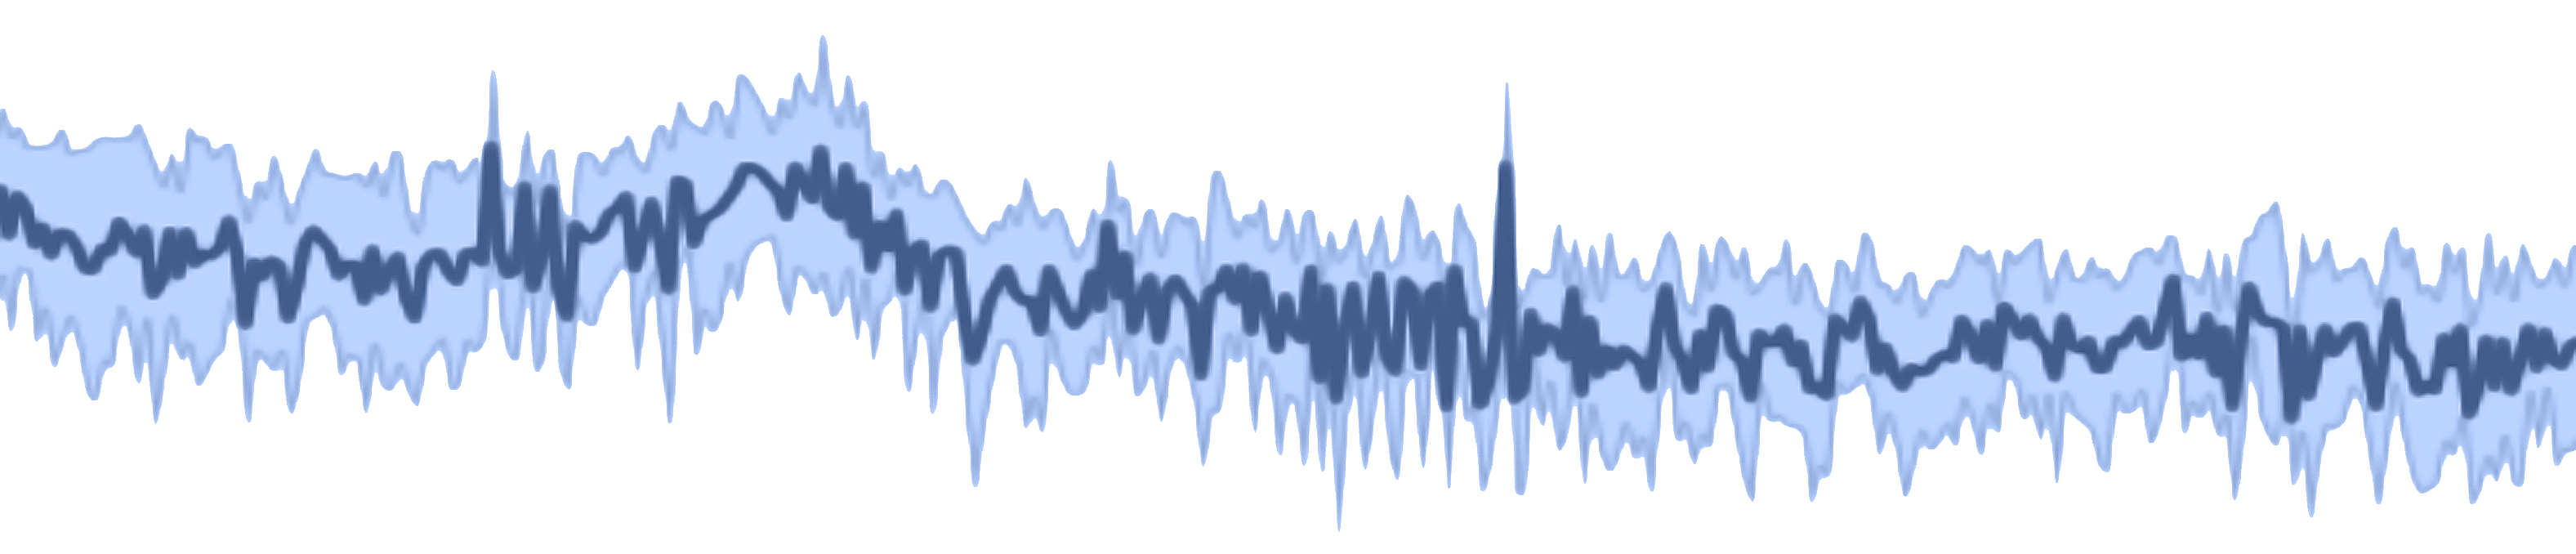
\includegraphics[width=17cm,keepaspectratio]{images/wave.png}}%
  }%
}

%\includeonly{chap-n}
\begin{document}

\begin{preface}
``I believe the future of communication is brain-computer interfaces''
\begin{flushright}
- Stephen Hawking \cite{hawking2018brief}
\end{flushright}

\end{preface}

\tableofcontents*

\begin{abstract}
  Brain-computer interfaces (BCIs) offer a promising means of communication and control for individuals with limited mobility due to neurological disorders or injuries. Steady-state visually evoked potentials (SSVEPs) are a type of BCI paradigm that rely on the brain's response to specific visual frequencies. Single frequency SSVEP suffers from the limited number of targets thus dual-SSVEP paradigms were proposed. Conventional dual-SSVEP paradigms, however, suffer from limitations such as intermodulation of harmonic components, which can result in reduced accuracy and reliability. 
  
  This study aims to explore the feasibility and effectiveness of a novel dual-SSVEP paradigm using virtual reality (VR) technology. By presenting SSVEP stimuli to each eye separately in a VR environment, we hypothesize that intermodulation of harmonic components can be mitigated, ultimately improving the accuracy and reliability of the SSVEP response. In this thesis, we design and implement a VR-based dual-SSVEP paradigm, evaluate its performance in terms of reliability, and compare its performance to a conventional dual-SSVEP paradigm.
\end{abstract}


\listoffiguresandtables
\chapter{List of Abbreviations and Symbols}
\section*{Abbreviations}
\begin{flushleft}
  \renewcommand{\arraystretch}{1.1}
  \begin{tabularx}{\textwidth}{@{}p{12mm}X@{}}
    BCI & Brain-Computer Interface \\
    BMI & Brain-Machine Interface \\
    EEG & Electroencephalogram \\
    ECoG & Electrocorticographic \\
    fMRI & Functional Magnetic Resonance Imaging \\
    fNIRS & Functional Near-Infrared Spectroscopy \\
    MEG & Magnetoencephalography \\
    PET & Positron Emission Tomography \\
    ITR & Information Transfer Rate \\
    SNR & Signal-to-Noise Ratio \\
    bpm & Bits per Minute \\
    c-VEP & Code-Modulated Visual Evoked Potentials \\
    t-VEP & Transient Visual Evoked Potentials \\
    ERP & Event-Related Potential \\
    SSVEP & Steady-State Visually Evoked Potential \\
    VR & Virtual Reality \\
    TCP   & Transmission Control Protocol \\
    LSL   & Lab Streaming Layer \\
    IP    & Internet Protocol \\
    PSD   & Power Spectral Density \\
    IM & Intermodulation \\
    BR & Binocular Rivalry \\
    FL & Focus Left \\
    FR & Focus Right \\
    
  \end{tabularx}
\end{flushleft}
\section*{Symbols}
\begin{flushleft}
  \renewcommand{\arraystretch}{1.1}
  \begin{tabularx}{\textwidth}{@{}p{12mm}X@{}}
    $f$   & Frequency \\
  \end{tabularx}
\end{flushleft}

% Now comes the main text
\mainmatter
\chapter{Introduction}
\section{Context and Motivation}
The human brain is one of the most complex and intriguing organs in the body, responsible for regulating a wide range of bodily systems and enabling us to engage in complex cognitive processes. With its billions of neurons and trillions of connections, it has captivated scientists for centuries \cite{bear2016neuroscience}.
A brain-computer interface (BCI), also referred to as a brain-machine interface (BMI), is a hardware and software communications system that enables humans to interact with their surroundings through control signals generated from electroencephalographic and  magnetoencephalographic activity. BCIs enable the translation of brain activity into commands that can be used to operate devices, such as computers or prosthetic limbs, eliminating the need of peripheral nerves and muscles \cite{wolpaw2012brain}.
BCI research is a relatively young multidisciplinary field integrating researchers from neuroscience, engineering, computer science, physiology, psychology, rehabilitation, and other technical and health-care disciplines \cite{wolpaw2012brain}.

Neural interfaces can be classified into two main categories based on the type of brain signal utilized for communication between the brain and the computer: invasive and non-invasive methods. Within these categories, there are three major classes of neural interfaces:
\begin{enumerate}
    \item Electroencephalographic (EEG) scalp electrode arrays: noninvasive attachment to the skin to record field potentials with low information content from widely distributed sets of neurons and synapses \cite{schwartz2004cortical}.
    \item Electrocorticographic (ECoG) electrode arrays: surgical positioning on the brain surface to record field potentials with moderate information content from localized sets of neurons and synapses \cite{schwartz2004cortical}.
    \item Miniaturized microelectrode arrays: surgical insertion into the cerebral cortex to record neuronal action potentials (spikes) from individual neurons and/or local field potentials (LFPs) from highly localized sets of neurons and synapses with high information content \cite{schwartz2004cortical}.    
\end{enumerate}

Non-invasive measurement techniques include functional magnetic resonance imaging (fMRI) \cite{glover2011overview}, functional near-infrared spectroscopy (fNIRS) \cite{chen2020functional}, magnetoencephalography (MEG) \cite{singh2014magnetoencephalography} and electroencephalography.
EEG is a non-invasive technique used to measure the electrical activity of the brain. EEG works by recording the electrical signals in the brain that are related to the flow of electric currents during synaptic excitation of neuronal dendrites, especially in the cortex, but also in the deep brain structures \cite{nicolasalonso2012brain} using electrodes placed on the scalp. These signals are amplified and processed to create a visual representation of the brain's activity, known as an EEG waveform or EEG trace \cite{bear2016neuroscience}. EEG-based BCI systems can be dated back to 1971, when a prosthetic arm was developed and could be controlled by EEG \cite{nirenberg1971new}. Since then, EEG has been widely studied to develop BCIs for controlling and communication \cite{birbaumer2007brain}.

The EEG waveform is characterized by different frequency bands, including delta ($<$ 4 Hz), theta (4-7 Hz), alpha (8-12 Hz), beta (12-30 Hz), and gamma waves (30-100 Hz). Each frequency band corresponds to a different level of brain activity, with delta waves representing deep sleep or unconsciousness, and gamma waves representing high-level cognitive processing \cite{schwartz2004cortical}.

EEG has several advantages over other brain imaging techniques, including its portability, low cost, high temporal resolution, and ability to measure brain activity in real-time \cite{niedermeyer2005electroencephalography}. However, it also has some limitations, such as its relatively low spatial resolution compared to techniques like fMRI and positron emission tomography (PET) \cite{luck2014introduction}.

Despite its limitations, EEG remains a valuable tool for studying the brain and has led to significant advances in our understanding of brain function. Ongoing research is focused on developing new EEG-based techniques for clinical diagnosis and treatment, as well as for cognitive enhancement and brain-computer interfaces \cite{mullerputz2005steadystate}.

Before diving into visual-based BCIs, it is important to understand some key performance metrics used to evaluate and compare different BCI systems. These metrics include accuracy, information transfer rate (ITR), signal-to-noise ratio (SNR), and user training requirements \cite{wolpaw2002brain}. Accuracy refers to the system's ability to correctly identify the user's intended command, while ITR measures the amount of information transmitted per unit of time, usually expressed in bits per minute (bpm). SNR represents the quality of the brain signal extracted by the BCI system, with a higher SNR indicating better signal quality and improved performance. Lastly, user training requirements reflect the ease of use and adaptability of a BCI system, with lower training requirements being more desirable for efficient and user-friendly interfaces \cite{kubler2007introduction}.

\begin{figure}
    \centering
    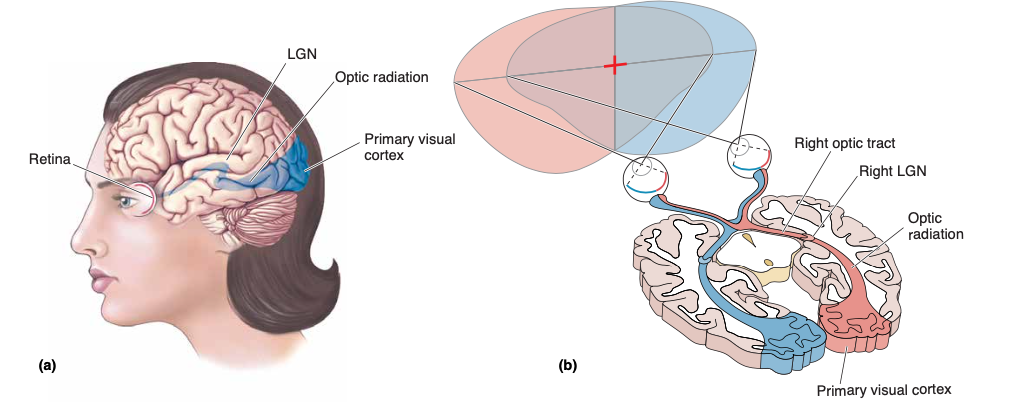
\includegraphics[width=0.75\textwidth]{images/intro/visual pathways.png}
    \caption{The visual pathway that mediates conscious visual perception. (a) A side view of the brain with the retinogeniculocortical pathway shown inside (blue). (b) A horizontal section through the brain exposing the same pathway(adapted from \cite{bear2016neuroscience}).}
    \label{fig:visual}
\end{figure}

To understand the foundation of visual-based BCIs, it's crucial to comprehend the basic visual pathway in humans which is shown in Figure \ref{fig:visual}. Light enters the eye through the cornea and is focused onto the retina, where it stimulates photoreceptor cells. These cells convert light into electrical signals, which are transmitted to the brain via the optic nerve. These signals first pass through the optic chiasm, where the information from the left and right visual fields are segregated. These segregated signals then travel through the lateral geniculate nucleus of the thalamus, where they are processed and sent to the primary visual cortex. This complex pathway allows for the detailed and nuanced visual processing that underlies our visual perception \cite{bear2016neuroscience}.

Building on the complexity of the visual pathway in humans, another intriguing aspect is the phenomenon of binocular vision and binocular rivalry. Binocular vision refers to the ability to integrate visual information from both eyes, providing depth perception and a more comprehensive view. Binocular rivalry, a subject of intensive investigation for over 160 years, occurs when dissimilar images are presented to corresponding regions of the two eyes. Rather than merging into a single view, the two images compete for perceptual dominance, with one image dominating conscious awareness for several seconds before being supplanted by the previously suppressed rival image. This rivalry reveals important grouping properties and provides a powerful tool for studying the neural concomitants of conscious visual awareness. The most recent evidence supports a view of rivalry as a series of processes, each implemented by neural mechanisms at different levels of the visual hierarchy, indicating the operation of nonlinear dynamical processes. This concept is foundational to understanding how the brain processes conflicting visual information and has implications for visual-based BCI systems \cite{blake2002visual}.

Visual-based BCI systems are a subset of brain-computer interfaces that specifically focus on utilizing the brain's visual processing capabilities to control external devices or communicate with the environment \cite{allison2007brain}. These systems often rely on the detection and interpretation of brain signals generated in response to visual stimuli, such as patterns, images, or flickering lights \cite{mullerputz2005steadystate}. As a result, visual-based BCIs can provide a more intuitive and user-friendly experience, allowing individuals to interact with their surroundings using natural visual attention and perception processes \cite{cecotti2011spelling}. Researchers continue to explore novel visual-based BCI paradigms to enhance system performance and usability, with the goal of developing practical applications for individuals with various needs, such as those with limited mobility or communication challenges \cite{guger2009many}.

The P300 paradigm, along with code-modulated visual evoked potentials (c-VEP) and transient visual evoked potentials (t-VEP), represents another approach in the field of visual-based BCIs \cite{wolpaw2012brain}. P300 is an event-related potential (ERP) characterized by a positive deflection in the EEG signal, typically occurring around 300 milliseconds after the presentation of a rare or unexpected stimulus \cite{sutton1965evoked}. Both c-VEP and t-VEP paradigms exploit the brain's response to specific visual stimuli, with c-VEP focusing on the rapid presentation of pseudorandom sequences \cite{sutter1992brain} and t-VEP capturing responses to sudden changes in the visual scene \cite{bin2009online}. While these methods have shown potential in BCI applications, the focus remains on the SSVEP paradigm.

SSVEP is a periodic brain electrical response induced by the repetitive presentation of a visual stimulus, flickering or reversing at a certain frequency ranging from 1 Hz to 60 Hz \cite{zhu2010survey}. The SSVEP-based BCI has many advantages over other BCI systems, including a higher SNR and ITR. Also, since the SSVEP is an inherent response of the brain, very little training is required to enable a person to operate the BCI \cite{bakardjian2010optimization}.

Although SSVEP can be elicited by a broad range of frequencies, the available frequencies in practical BCI applications are often restricted by several factors. First, all available stimulation frequencies do not always evoke high SSVEP responses. The frequencies that elicit strong SSVEP responses are highly dependent upon the participants, as well as various properties of the visual stimuli, such as color, size, and contrast \cite{zhu2010survey}. Second, the use of two frequencies, $f_1$ and $f_2$, in the same experiment has been typically avoided when $f_1$ is a multiple of $f_2$ or vice versa because of the harmonic SSVEP responses \cite{cheng2002design,shyu2010development,wang2017benchmark}.
\begin{figure}
    \centering
    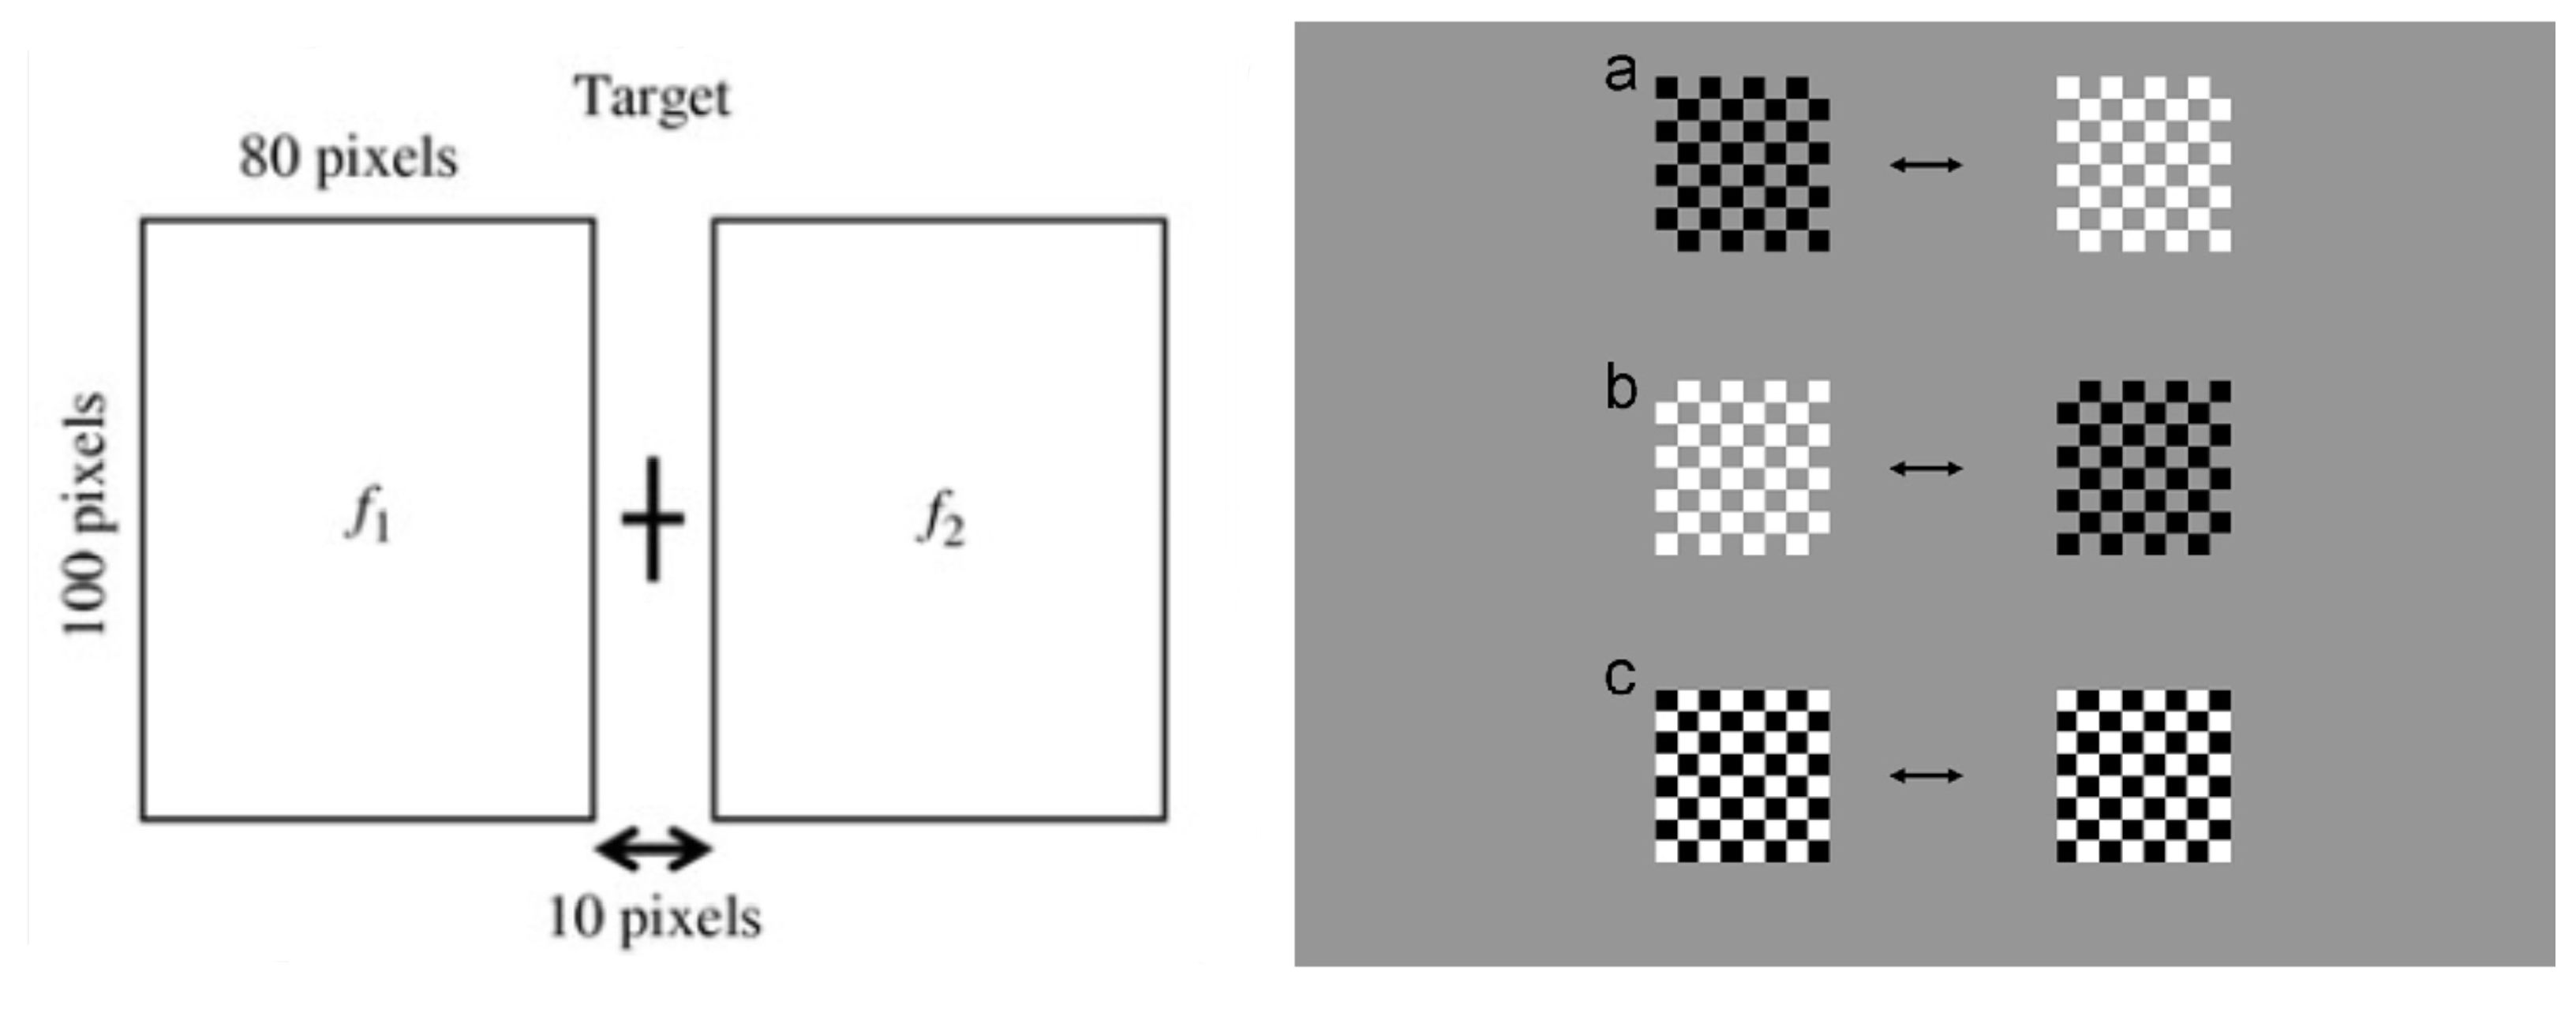
\includegraphics[width=0.75\textwidth]{images/intro/dual.png}
    \caption{Composite image showing the left-right view paradigm (adapted from \cite{yan2011right}) and the checkerboard paradigm (adapted from \cite{hwang2013new}).}
    \label{fig:dual}
\end{figure}
Dual-SSVEP paradigms have been developed to address some of the limitations of single-frequency SSVEP systems. In a dual-SSVEP paradigm, two different frequencies, $f_1$ and $f_2$, are simultaneously presented to the user, typically using one of two methods: the left-right view paradigm or the checkerboard paradigm \cite{vialatte2010steadystate,mullerputz2008control}. Figure \ref{fig:dual} illustrates these two paradigms, with the left-right view paradigm shown on the left and the checkerboard paradigm on the right.

In the left-right view paradigm, each frequency is presented in a distinct spatial location, usually with $f_1$ in the left visual field and $f_2$ in the right visual field. The user can select one of the multiple targets by focusing their attention on the fixation point. This approach does not merely double the number of available targets, as initially suggested, but actually increases the number of potential targets combinatorially. Given $n$ different frequencies, the number of potential targets is of the form $C_{n2}$ (combinations of $n$), since two frequencies can be used simultaneously \cite{mullerputz2008control,zhang2015toward,min2014neuroimaging,friman2009spelling}. Furthermore, this paradigm enhances the robustness of the BCI by reducing the impact of transient attentional shifts and visual fatigue, which can affect the performance of single-frequency SSVEP systems \cite{mullerputz2008control,zhang2015toward,min2014neuroimaging,lin2007frequency}.

The checkerboard paradigm, on the other hand, involves presenting the two target frequencies as alternating squares in a checkerboard pattern. This arrangement allows the user to focus on the entire visual field, and the response of the brain to the target frequencies can be selectively attended to and decoded by the BCI system \cite{min2014neuroimaging,cao2020highperformance,chen2015filter}. The checkerboard paradigm has been shown to improve the stability of the SSVEP response and increase the ITR compared to the left-right view paradigm \cite{min2014neuroimaging,cao2020highperformance,pan2011detecting}.

Overall, both the left-right view and checkerboard paradigms offer advantages over single-frequency SSVEP systems. They increase the number of control commands without increasing the visual complexity of the interface, making them more attractive for practical applications \cite{lin2017frequency,mullerputz2005steadystate}. Moreover, by exploiting the brains natural ability to selectively attend to different visual stimuli, dual-SSVEP paradigms can provide a more intuitive and user-friendly BCI experience \cite{trenado2019enhancing,bin2011vepbased}.

Despite its potential advantages, dual-SSVEP systems still face some challenges \cite{cheng2002design,shyu2010development,wang2017benchmark}. One major issue faced by dual-SSVEP systems is the unpredictable intermodulation (IM) of the harmonic components \cite{sun2023binocular}. Intermodulation components arise when different elements of a stimulus are modulated using more than one frequency, leading to neural responses not only at the original frequencies but also at additional frequencies. These IM components result from the non-linear integration of neural signals driven by differentially modulated stimulus elements. IM components have been used in frequency tagging neuroimaging designs and have emerged as a promising direct measure of neural interactions. They have initially been used to investigate low-level visual processing and are now being applied to study mid- and high-level perceptual processes, including the involvement of cognitive functions such as attention and expectation. IM components provide direct evidence for non-linear interactions within the visual pathways and offer insights into the existence, degree, and type of neural integration mechanisms at hand \cite{gordon_intermodulation_2019}.

\section{Problem Statement}

In recent years, research into BCIs has gained significant interest as a means of providing communication and control for individuals who have lost the ability to move or speak due to neurological disorders or injuries. One promising type of BCI is the SSVEP, which utilizes the brain's response to visual stimuli presented at specific frequencies to communicate information. However, conventional dual-SSVEP paradigms have certain shortcomings, such as intermodulation of harmonic components, which can lead to reduced accuracy and reliability of the SSVEP response.

To address these shortcomings, a novel binocular dual-SSVEP paradigm in a polarized display system was recently proposed \cite{sun2023binocular}, according to which, Information Transfer Rate (ITR) can be increased, and noise can be reduced compared with traditional dual-SSVEP paradigms. However, the polarized-light system used in the study is rather impractical to use in daily life. Therefore, the present study aims to evaluate a novel dual-SSVEP paradigm using virtual reality (VR) technology. VR has several benefits for BCI applications, such as the ability to control what each eye sees individually, providing more control of what the user sees and greater immersion. By utilizing VR to present the SSVEP stimuli to each eye separately, it may be possible to remove the IM of harmonic components and improve the accuracy and reliability of the SSVEP response.

The goal of this thesis is to evaluate the feasibility and effectiveness of this new dual-SSVEP paradigm in a VR environment. The specific objectives are to design and implement a VR-based dual-SSVEP paradigm, evaluate the paradigm's performance in terms of accuracy and reliability of the SSVEP response using the power spectral density (PSD) as a metric, and compare the performance of the VR-based dual-SSVEP paradigm to that of a conventional dual-SSVEP paradigm.

\subsection{Research Questions}

Building on the identified limitations of conventional dual-SSVEP paradigms, this study aims to explore the efficacy of a VR-based approach in enhancing the accuracy and reliability of SSVEP responses.
The research is guided by several key questions, as outlined in Table \ref{tab:comparisons} below. Overall, the proposed study has the potential to significantly advance the development of SSVEP-based BCIs by addressing the shortcomings of conventional dual-SSVEP paradigms and improving the accuracy and reliability of the SSVEP response. By utilizing VR technology, the study may also provide new insights into the neural mechanisms underlying SSVEP responses and the role of visual processing in BCI applications.

\begin{landscape}
    \begin{table}
    \centering
    \begin{tabularx}{\linewidth}{>{\centering\arraybackslash}p{0.75cm}>{\centering\arraybackslash}p{3.5cm}>{\raggedright\arraybackslash}X>{\raggedright\arraybackslash}X}
        \hline
        
        \textbf{Exp.} & \textbf{Conditions} & \textbf{Research Question} & \textbf{Null Hypothesis} \\
        
        \hline
        \addlinespace
        1 & L$f_{1}$R$\varnothing$ vs. L$f_{1}$R$f_{1}$ vs. L$\varnothing$R$f_{1}$ & 
        Can we differentiate hemisphere-specific SSVEP responses based on the visually stimulated eye? & There is no difference in SSVEP responses or hemisphere-specific activity regardless of which eye is stimulated. \\
        \addlinespace
        \addlinespace
        \addlinespace
        2 & L$f_{1}$R$f_{2}$ vs. L$f_{2}$R$f_{1}$ & 
        Can we differentiate SSVEP responses based on the unique frequency stimuli presented to each eye? & SSVEP responses cannot be differentiated based on the unique frequency stimuli presented to each eye. \\ 
        \addlinespace
        & & Can we simultaneously elicit separate SSVEP responses in both hemispheres? & Separate SSVEP responses cannot be simultaneously elicited in both hemispheres. \\
        \addlinespace
        4 & \makecell{(FL - BR L$f_{2}$,~R$f_{1}$)\\vs.\\(FR - BR L$f_{2}$,~R$f_{1}$)} & Can the direction of participants' attention control or influence binocular rivalry? & The direction of participants' attention has no control or influence over binocular rivalry. \\
        \addlinespace
        \hline
    \end{tabularx}
    \caption{Overview of the experimental comparisons and the associated research questions.}
    \emph{Note: In the notation, L$f_{1}$R$\varnothing$ represents the left eye seeing frequency $f_{1}$ and the right eye seeing no stimulation (absence denoted by "$\varnothing$"). Similarly, L$f_{2}$R$f_{1}$ represents the left eye seeing frequency $f_{2}$, and the right eye seeing frequency $f_{1}$. \\
    BR = Binocular Rivalry; FL/FR = Focus Left/Right}
    \label{tab:comparisons}
\end{table}
\end{landscape}

\section{Literature Review}

SSVEPs driven BCIs are a significant area of research. The focus of this literature review is on the challenges and advancements in dual-frequency SSVEPs, particularly in the context of the proposed novel dual-SSVEP paradigm using VR technology.

Hwang et al. \cite{hwang2013new} introduced a novel dual-frequency stimulation method to increase the number of visual stimuli for multi-class SSVEP-based BCIs. This approach overcame the "attention-shift" problem by using a single visual stimulus mixed with two different patterns. The method utilized a conventional black-white checkerboard pattern and generated ten visual stimuli by combining four different stimulation frequencies. The implementation of a mental keypad system using this method reported an average information transfer rate of 33.26 bits/min and an average accuracy of 87.23\%. The hypothesis of this paper was that the dual-frequency stimulation method could enhance the number of visual stimuli without increasing complexity. The study also highlighted the importance of the selection of stimulation frequencies and the design of visual stimuli, which are directly related to the aim of the current study.

Chen et al. \cite{chen2015filter} developed a filter bank canonical correlation analysis (FBCCA) method to enhance SSVEP detection. The paper introduced three methods (M1, M2, M3) for optimizing filter bank design, each with different sub-band decompositions. The FBCCA methods were compared with the standard CCA method for classification accuracy and ITR. Method M3 achieved the highest classification performance, and an online BCI speller using the optimal FBCCA method achieved an average ITR of \(151.18 \pm 20.34\) bits min\(^{-1}\). The assumption in this paper was that incorporating fundamental and harmonic SSVEP components would improve detection. The study also discussed the importance of the spatial filter design and the need for individual calibration, aligning with the focus of the current study on improving accuracy and reliability.

Yan et al. \cite{yan2011right} proposed a right-and-left visual field stimulation technique where each visual stimulus was characterized by a spatial frequency and a temporal frequency. This approach significantly increased the number of possible commands without increasing the number of visual stimuli. The paper identified challenges such as the complexity of visual stimuli and the likelihood of IM components. The hypothesis of this paper was that a right-and-left visual field stimulation technique could enhance command possibilities without increasing stimuli. The study also explored the use of different algorithms for frequency recognition and the potential for user-specific customization, providing insights into the focus of this current study on novel dual-SSVEP paradigms.

Sun et al. \cite{sun2023binocular} introduced a novel binocular dual-SSVEP  paradigm utilizing a polarized display system. The primary objective of their research was to enhance the ITR and minimize noise, thereby improving upon traditional dual-SSVEP paradigms. Their hypothesis posited that a binocular approach could significantly improve ITR while reducing noise, although they acknowledged the current technological limitations as a constraint. 

The study is particularly noteworthy for its comprehensive experimental design, which included two key experiments. The first, a 6-target offline experiment, demonstrated a 2 dB increase in the SNR of target frequency components when compared to unpredictable IM components. This result indicates a more stable and reliable signal, which is crucial for the practical application of BCI. The second experiment was an online 40-target test that yielded an average ITR of \(104.56 \pm 15.74\) bits/min. Remarkably, this rate is nearly double that of existing dual-frequency paradigms, underscoring the efficacy of their novel approach.

Furthermore, Sun et al. contributed to the algorithmic aspect by introducing an improved filter bank dual-frequency canonical correlation analysis (FBDCCA). This algorithm is tailored for dual-frequency SSVEP paradigms and serves to further optimize the system's performance. In addition to these technical contributions, the paper also delved into the spatial separation of visual stimuli and explored the potential for integrating other sensory modalities. While the study is a significant step forward, it also highlights the impracticality of the current technology as a limitation. The current research aims to evaluate a similar dual-SSVEP paradigm but leverages Virtual Reality technology, potentially overcoming some of these limitations.

\chapter{Materials and Methods}
\label{cha:methods}

\section{Participants}
The study included eight participants (five males, three females) with an age range of 19 to 25 years (mean = 21.75 years, SD = 2.05 years). None of the participants suffered from any neurological disease or were on any medication. Participant recruitment was primarily conducted through referrals from acquaintances and fellow students of the university. 

To be included in the study, participants had to meet the following criteria: be between 18 and 30 years of age, have normal or corrected-to-normal vision, and not have a history of photosensitive epilepsy, migraines, or other neurological disorders. 

The exclusion criteria for the study were as follows: any visual impairment that cannot be corrected with glasses or contact lenses, any neurological disorder that may affect the participant's ability to complete the experiment, any condition that may increase the risk of photosensitive epilepsy or adverse reactions to flickering stimuli, and any condition that may affect the participant's ability to provide informed consent. 

Prior to the experiments, all participants provided signed consent indicating their understanding of the study's objectives and procedures and their voluntary agreement to participate. The study was conducted at the Laboratory for Neuro-and Psychophysiology, Department of Neurosciences, KU Leuven. The study was previously approved by the Ethics Commission Research UZ/KU Leuven, under registry number B322201940585 (communication code: S62547), approved on 7 June 2019.

\section{Data Acquisition}
The experiment utilized a Meta Quest Pro VR headset~\cite{meta} to present the visual stimuli and a Mentalab Explore~\cite{mentalab}, 8-channel, dry-electrode, wireless EEG system for recording the  brain activity of the participants. The VR headset allowed us to show different stimuli to each eye, and it provided an immersive environment.

% insert images/EEG-1020.png
\begin{figure}[ht]
    \centering
    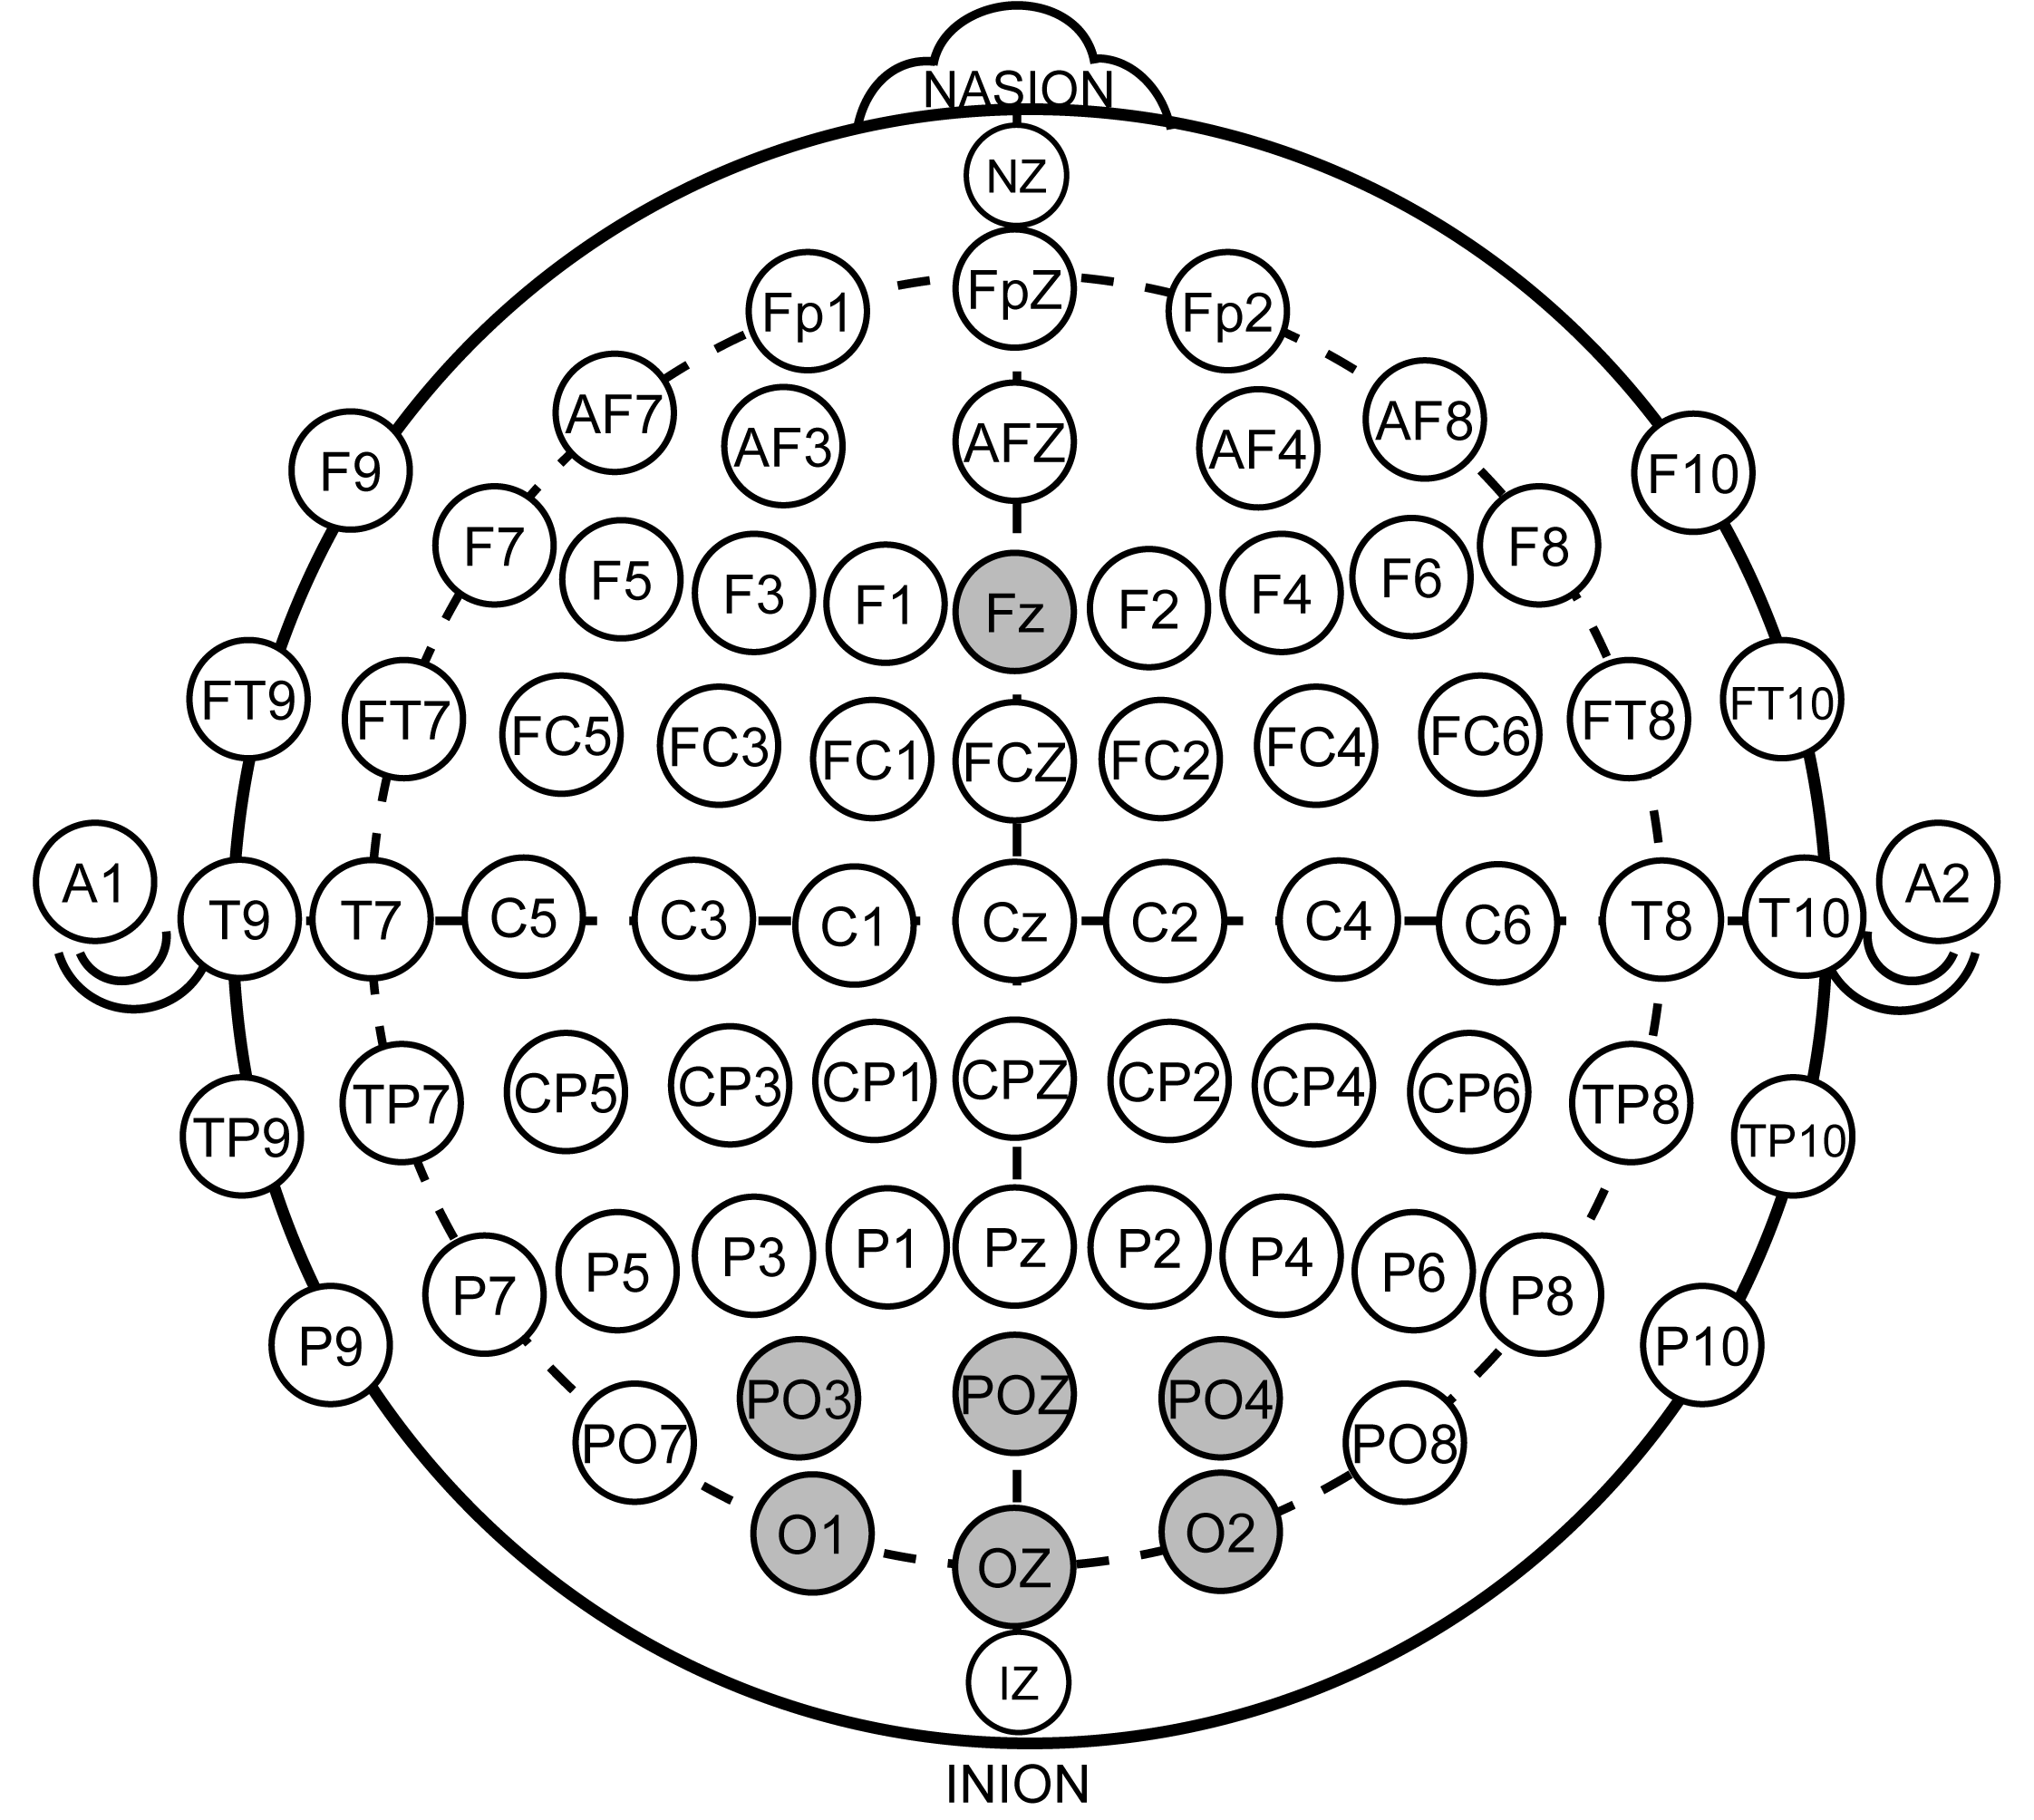
\includegraphics[width=0.45\textwidth]{images/methods/EEG-1020.png}
    \caption{EEG 10--20 System, highlighting the six electrodes and the ground reference used.}\label{fig:EEG-1020}
\end{figure}

Six of the eight electrodes were placed based on the international 10--20 system, specifically on the PO3, POz, PO4, O1, Oz, and O2 channels as illustrated in Figure~\ref{fig:EEG-1020}, while the ground electrode was placed on Fz. The remaining two electrodes were not used due to technical issues. Conductive gel was applied to ensure proper contact between the electrodes and the scalp, which resulted in optimal signal quality. The entire EEG setup process, including electrode placement and application of conductive gel, took approximately 45--60 minutes.

The EEG data was recorded and stored at a sampling rate of 250 Hz using a Python script with the Mentalab library. The refresh rate of the VR screens were set at the maximum of 90 Hz.

% add figure 
\begin{figure}[ht]
    \centering
    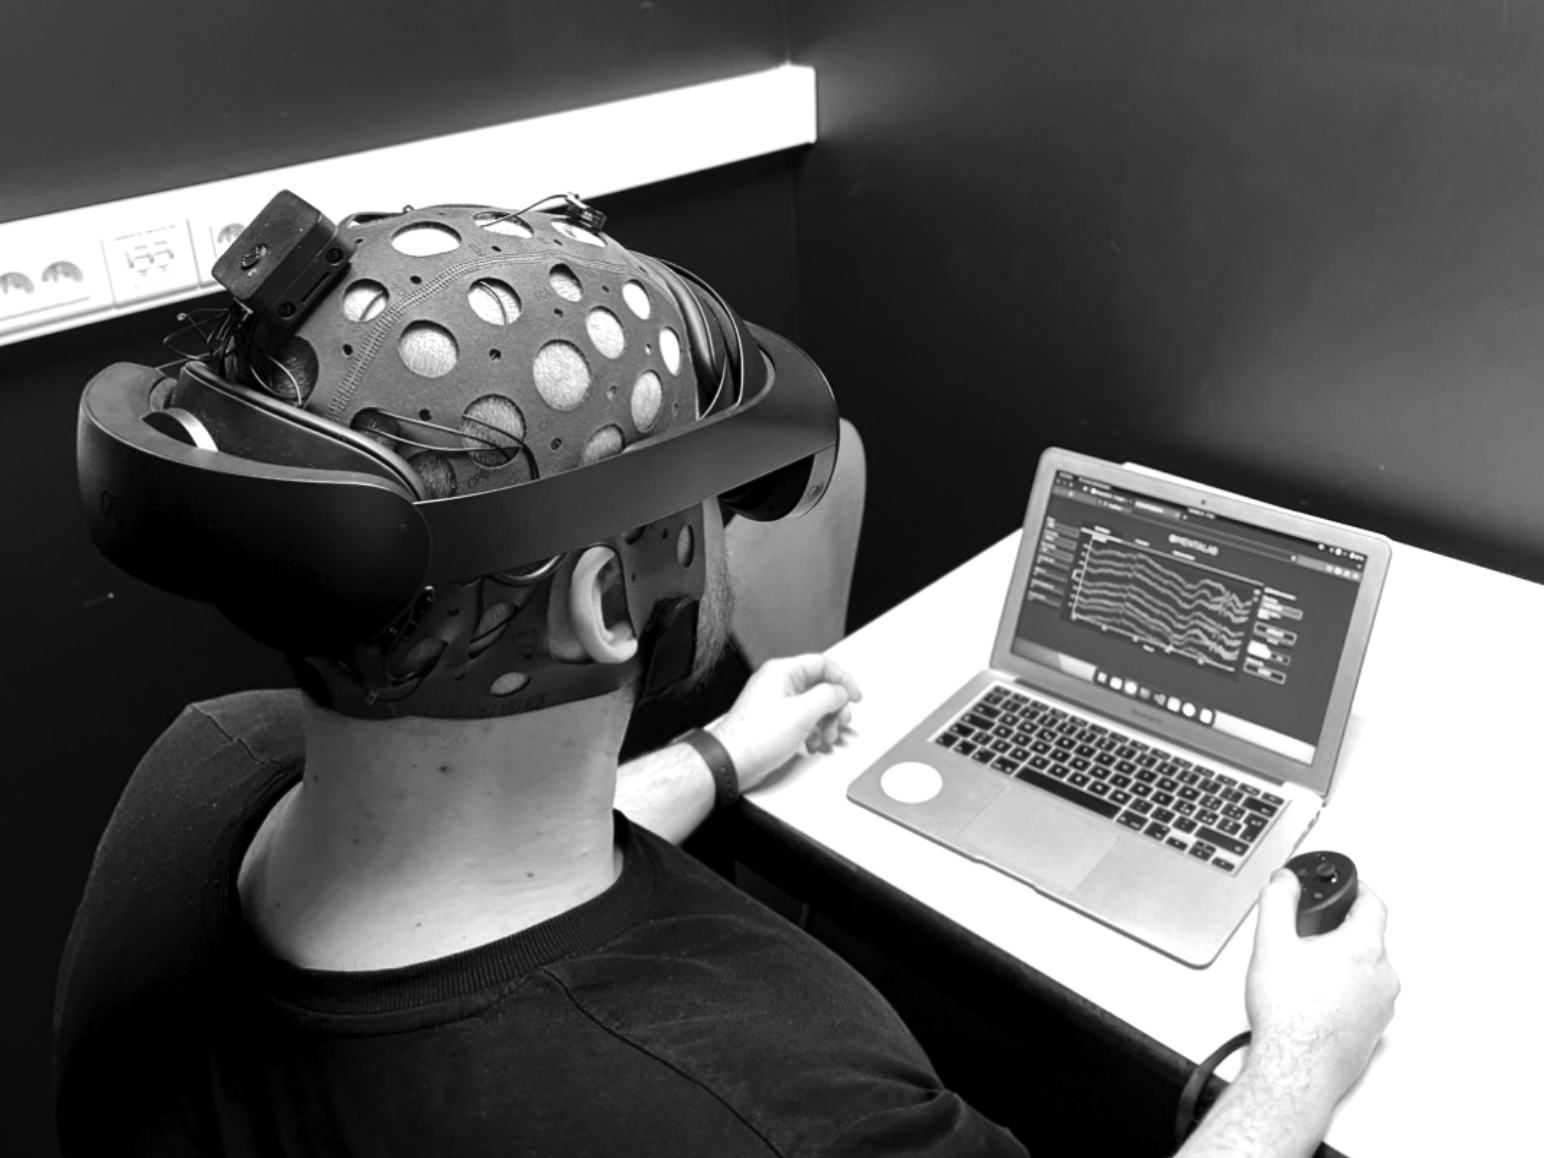
\includegraphics[width=0.5\textwidth]{images/experiments/experiment_setup.png}
    \caption{Experimental setup configuration depicted in the image. The VR controller is on the right hand, on top of the table to minimise movement.}\label{fig:mentalab}
\end{figure}

\section{Application Design}

The application design consists of two main components: the VR Experiment Application and the Transmission Control Protocol (TCP) Server. This allows easy communication and accurate markers synchronization between the VR headset, the laptop server, and the Mentalab system, using the TCP and Lab Streaming Layer (LSL) protocols.

\subsection{VR Experiment Application}


\begin{figure}[b]
    \centering
    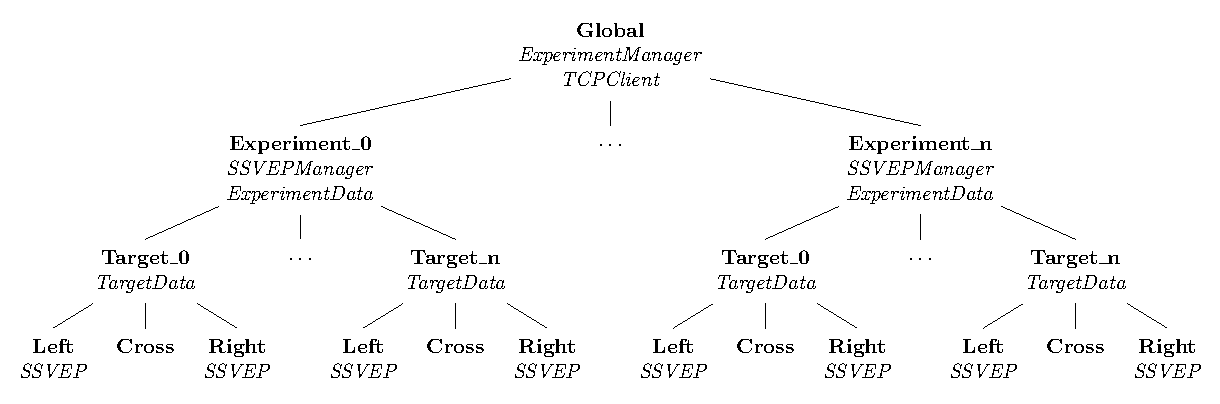
\includegraphics[width=\textwidth]{images/methods/hierarchy.pdf}
    \caption{Unity Scene for the VR Application, with the GameObjects in bold and their Scripts in italics.}\label{fig:unity-scene}
\end{figure}



The VR Experiment Application is a Unity project designed for Meta Quest devices, which comprises multiple experiments with multiple targets. The application is managed by a Global GameObject that communicates with the server through TCP/IP, allowing for the exchange of data, including markers, from the VR application to the laptop server in real-time. The application consists of several components, as illustrated in Figure~\ref{fig:unity-scene}. \\

The game objects are as follows:

\texttt{- Global}: Responsible for the TCPCLient and ExperimentManager scripts.

\texttt{- Experiment}: Responsible for the ExperimentData and SSVEPManager scripts.

\texttt{- Target}: Contains the Left and Right game objects.

\texttt{- Left/Right}: These are the patterns that flicker at the specified frequency. Left is presented to the left eye, and right is presented to the right eye.

\texttt{- Cross}: The cross guides the participant's gaze to the center of the target. 
\\

The scripts are as follows:

\texttt{- TCPClient}: Establishes the TCP connection and manages the communication.

\texttt{- ExperimentManager}: Cycles through the experiments.

\texttt{- ExperimentData}: Manages the experiment's visibility and the target status.

\texttt{- SSVEPManager}: Controls the start and pause of SSVEP components.

\texttt{- TargetData}: Manages the visibility of the Cross object within each target.

\texttt{- SSVEP}: Controls the flickering using a square wave with the specified frequency, as illustrated in Figure~\ref{fig:SSVEP}.

\begin{figure}[ht]
    \centering
    \includegraphics[width=0.65\textwidth]{images/methods/SSVEP.pdf}
    \caption{Black and white checkerboards contrast reversed at 6.6Hz with a square wave (adapted from the supplemental information of~\cite{ZHANG2011362}).}
    \label{fig:SSVEP} 
\end{figure}

\subsection{TCP Server and LSL Integration}

The TCP Server is a Python-based server that listens for client connections on a specific IP address and port. Once the data is received by the laptop server, it is then parsed, and forwarded to the EEG system using the LSL~\cite{lsl} protocol. LSL is an open-source networked middleware ecosystem designed to synchronize various experimental recording streams, including neural data. This protocol is also supported by the Mentalab system.

The markers consisted of a three-digit code. The first digit indicated whether the SSVEP was resumed (1) or paused (2). The second digit represented the experiment number, and the third digit denoted the target within the experiment, starting from the left. For example, 110 corresponded to the start of the leftmost target in the second experiment.

\section{Experiment Design}
In total, four experiments were designed to investigate the research questions in Table \ref{tab:comparisons}. The experiments included multiple targets with different frequencies, presented separately to the left and right eyes. The stimulus pattern design was developed based on previous studies \cite{ZHANG2011362, DavidCarmel2010, yan2011right, hwang2013new, vialatte2010steadystate}, ensuring optimal stimulation of the visual cortex. This included the checkerboard design, the use of a square wave instead of sine, and the color of the checkerboards for the binocular rivalry. 

The stimuli consisted of square wave patterns, with luminance control to maintain consistent brightness. The choice of frequencies (6.6 Hz and 7.5 Hz) was based on previous studies, which have demonstrated their effectiveness in eliciting robust SSVEP responses. Each experiment followed a similar structure of 6-second SSVEP periods and 3-second breaks, repeated ten times per target for a total duration of 90 seconds per target. 


\subsubsection{Experiment 1}
This experiment involved three targets: left, middle, and right, each displaying a black and white checkerboard pattern with the contrast reversed at 7.5 Hz ($f_{1}$) using a square wave, similar to the Figure~\ref{fig:SSVEP}. The left target was visible to the left eye only (L$f_{1}$R$\varnothing$), the middle target was visible to both eyes (L$f_{1}$R$f_{1}$), and the right target was visible to the right eye only (L$\varnothing$R$f_{1}$). 

The objective was to determine if SSVEP responses could be differentiated based on which eye saw the target (left, right, or both) and if it was possible to discern which eye saw it. If successful, this approach could enable the use of three targets with just one frequency.


\begin{figure}[h]
    \centering
    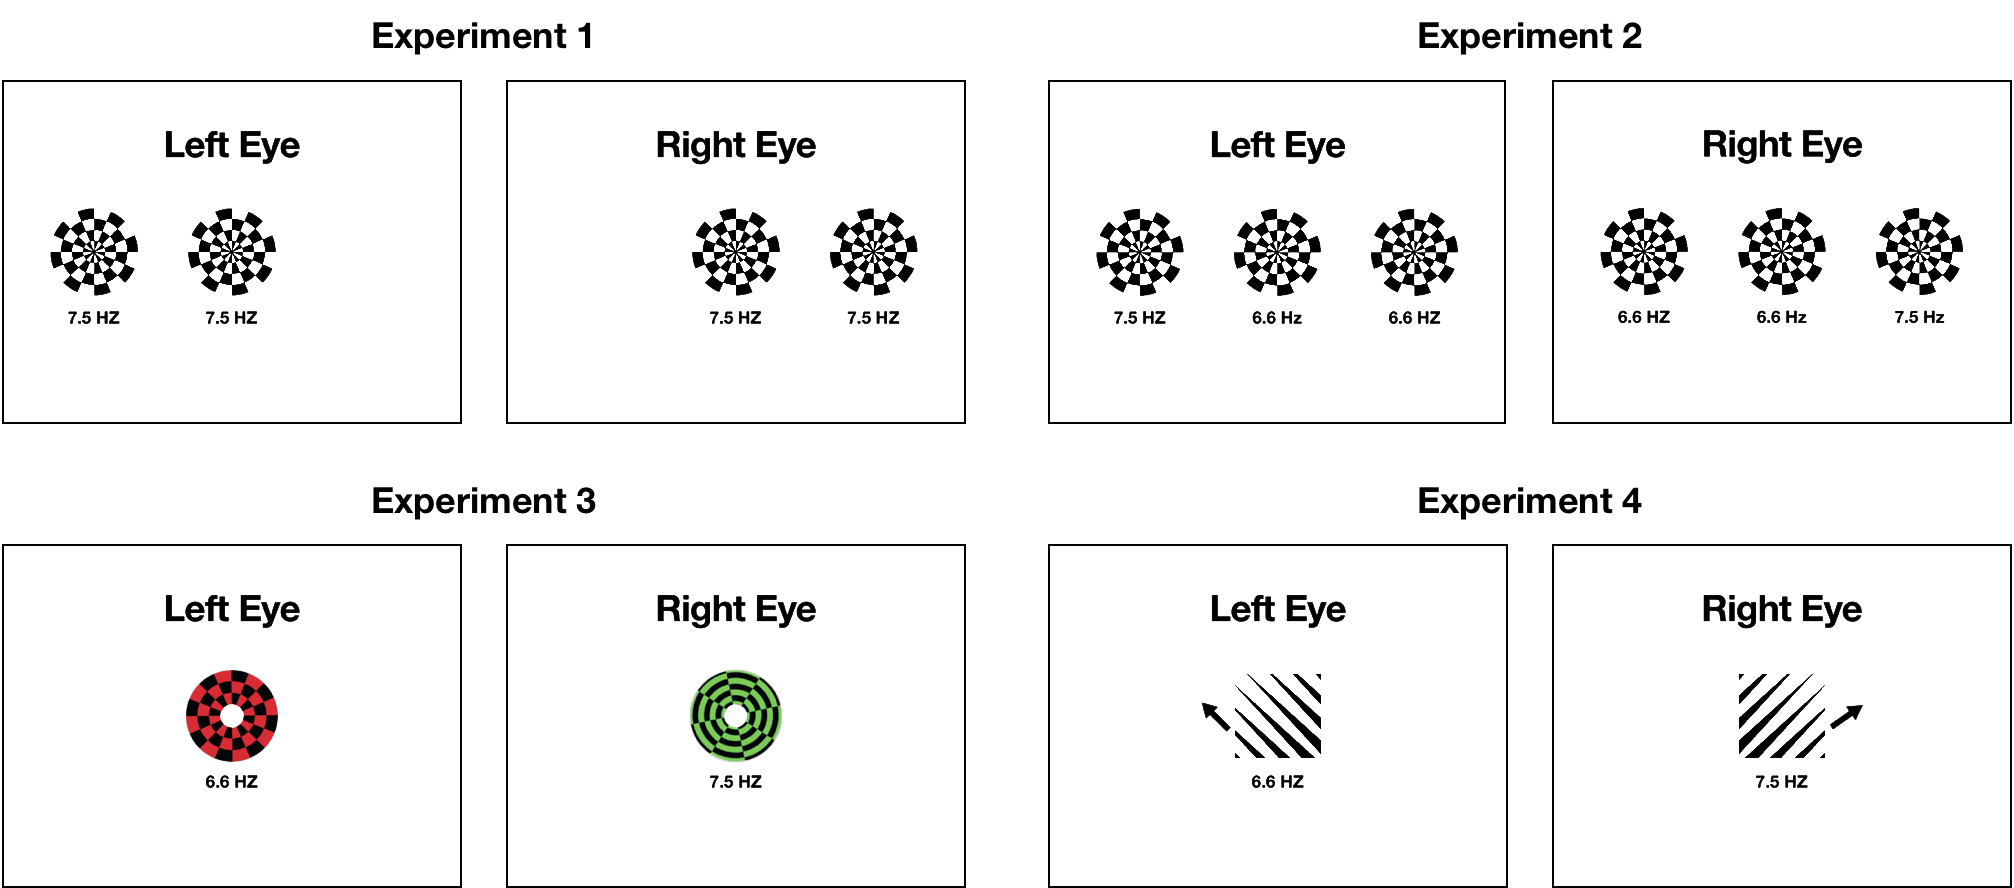
\includegraphics[width=1.0\textwidth]{images/experiments/experiments_w.png}
    \caption{Experiment Guide.}
    \label{fig:experiments}
\end{figure}

% insert figure
\begin{figure}[h]
    \centering
    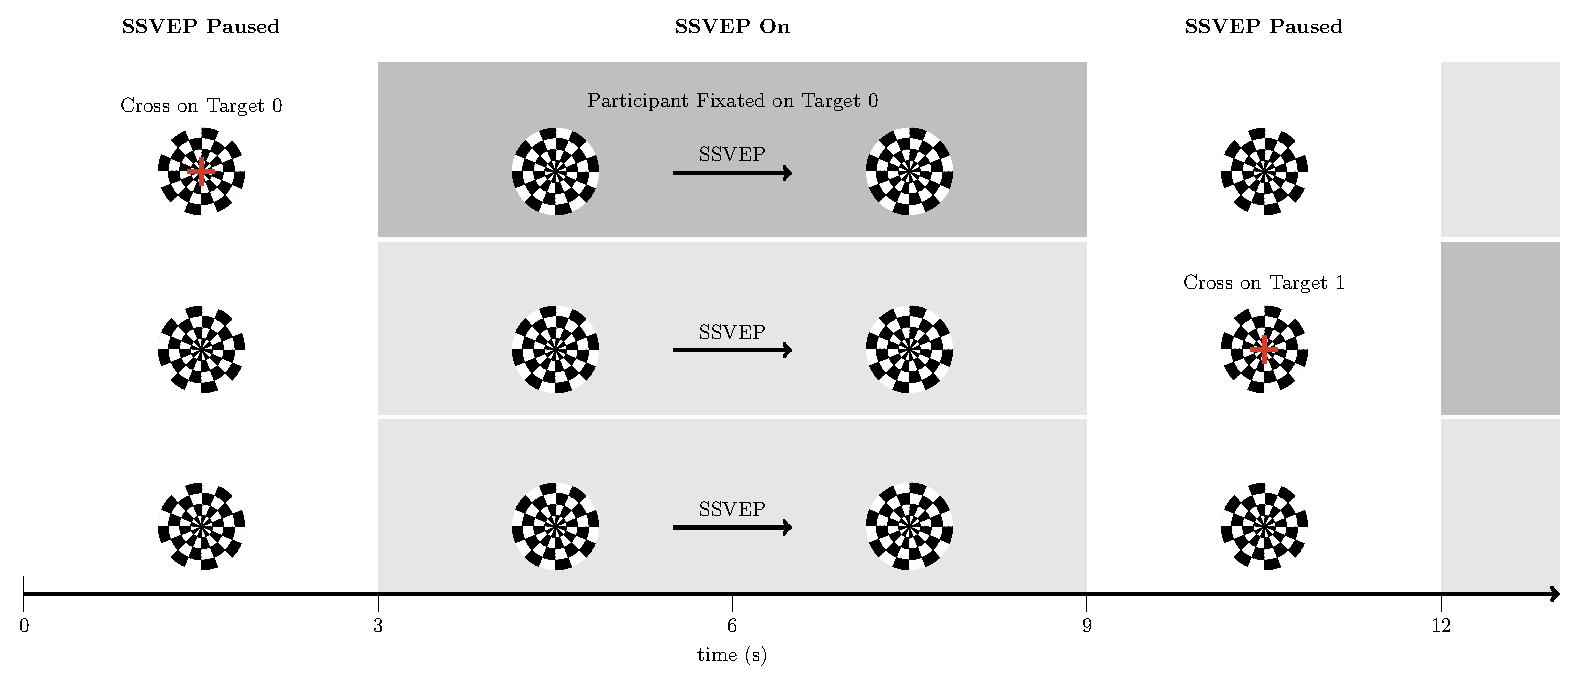
\includegraphics[width=1.0\textwidth]{images/methods/timing.pdf}
    \caption{Illustration of the Timing Graphs for Experiment 1 and Experiment 2.}
    \emph{Throughout this process, we cycled through the patterns illustrated in the figure in a circular manner, conducting 10 trials for each target. A trial was defined as the period between 3 and 9 seconds after the initial appearance of the cross above the respective target. The three targets were positioned side by side, as shown in Figure~\ref{fig:experiments}}
    \label{fig:experiment-timing}
\end{figure}

\subsubsection{Experiment 2}
In this experiment, three targets were presented: left, middle, and right, each displaying a black and white checkerboard pattern. For the left target, the left eye viewed the pattern at 7.5 Hz ($f_{1}$), while the right eye perceived it at 6.6 Hz ($f_{2}$). Conversely, for the right target, the left eye viewed the pattern at $f_{2}$, and the right eye at $f_{1}$. The middle target acted as a reference, flickering at $f_{2}$ for both eyes, in contrast to Experiment 1, where the middle target flickered at $f_{1}$ for both eyes.

The objectives of this experiment were twofold: first, to examine whether the left target (L$f_{1}$R$f_{2}$) could be distinguished from the right target (L$f_{2}$R$f_{1}$) based on the frequency differences perceived by each eye. Second, to assess if two separate SSVEP responses could be simultaneously elicited in both hemispheres. Experiment 2 expands upon Experiment 1, which involved one frequency in one eye and nothing in the other eye.

\subsubsection{Experiment 3}

This experiment served as a preliminary test to assess the feasibility of inducing binocular rivalry in a virtual reality setting. Inspired by the study "Binocular Rivalry Requires Attention," \cite{ZHANG2011362}, it aimed to examine the role of attention in binocular rivalry by presenting a single target with differing stimuli for each eye. The right eye viewed green checkerboards with the contrast reversed at 6.6 Hz (L$\varnothing$R$f_{2}$), while the left eye saw red checkerboards reversed at 7.5 Hz (L$f_{1}$R$\varnothing$). This experiment served as a foundational building step for the subsequent experiment.

\subsubsection{Experiment 4}

Building on the findings of Experiment 3, this final experiment aims to expand on the work done by the paper "Binocular Rivalry Requires Attention" \cite{ZHANG2011362}. Specifically, it assesses the impact of directed attention on binocular rivalry. Participants were instructed to focus on a specific image, as indicated by an arrow pointing in one of the pattern directions during the three-second break before each trial.

In this experiment, a single target was presented, featuring a pattern with white and black spikes rotated at 45 degrees. The spikes were thicker in the middle than on the sides. The left eye viewed the pattern at 6.6 Hz (L$f_{2}$R$\varnothing$), while the right eye saw the same but mirrored pattern at 7.5 Hz (L$\varnothing$R$f_{1}$).

\clearpage
\begin{figure}
    \centering
    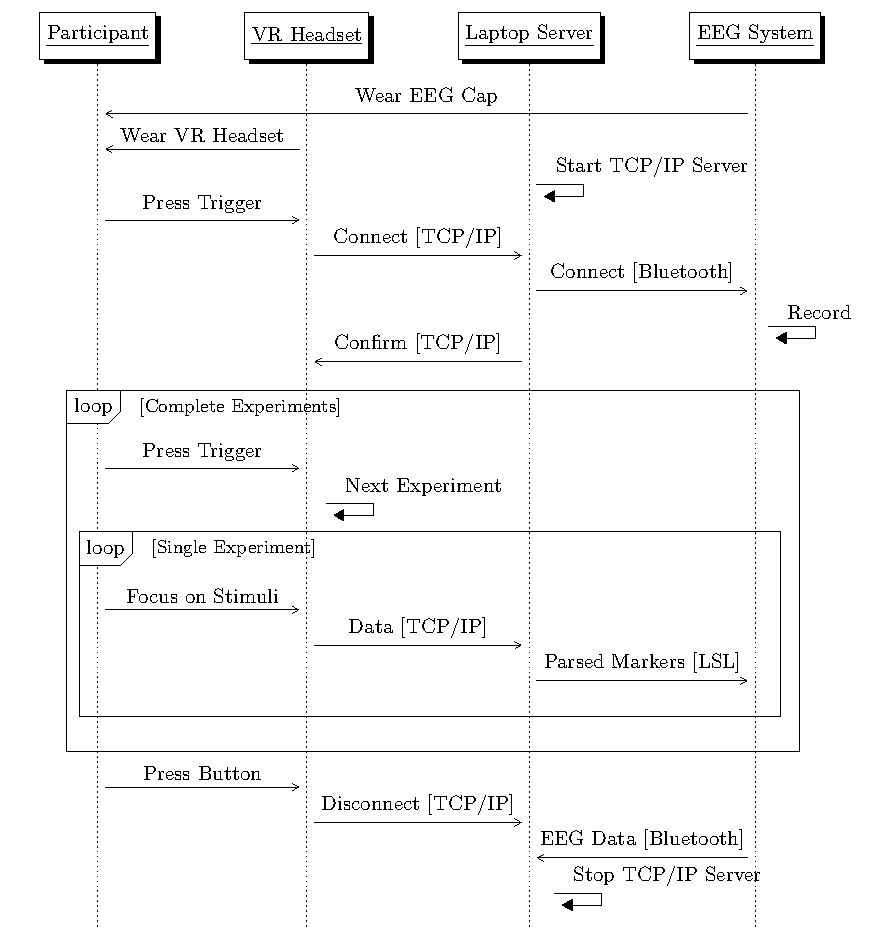
\includegraphics[width=1\textwidth]{images/methods/procedure.pdf}
    \caption{Experimental Procedure.}\label{fig:procedure}
\end{figure}
\clearpage

\section{Experimental Procedure}
Before the experiment, participants were provided with written and verbal instructions explaining the tasks they would perform during the experiment. They were informed about the use of the VR headset and the EEG cap, as well as the purpose of the study. Participants were encouraged to ask questions and clarify any concerns before the experiment began.

The experimental procedure, as illustrated in Figure~\ref{fig:procedure}, consists of several steps involving the participant, the VR headset, the laptop server, and the EEG system. The sequence diagram provides a visual representation of the interaction between these components. Participants were fitted with an EEG headset, followed by wearing the VR headset after ensuring a high-quality clean signal. The TCP server was initiated in the laptop. Participants initiated the connection by pressing the index trigger of the VR controller. A confirmation was sent from the laptop server once both the participant and the researchers were ready.

During the experiment, participants were instructed to focus on flickering stimuli, without moving their head or jaw. Upon completion of each experiment, the participant pressed the trigger to begin the next experiment. This process was repeated until all experiments were completed. The entire procedure was then repeated again. 

Participants were given short breaks of one to three minutes between experiments to minimize fatigue and maintain their focus throughout the experiment. The total duration of the experiment, including breaks, was approximately 45 minutes.

Upon completion of the experiment, participants were given a brief questionnaire to gather subjective feedback on their experience with the VR environment, their ability to focus on the stimuli, and any discomfort or adverse reactions they may have experienced during the experiment.

\section{Data Analysis}

\subsection{Preprocessing}

The signals from the six electrodes were filtered using a fourth-order Butterworth bandpass filter from 3 Hz to 100 Hz. Common average referencing was applied to remove common noise sources by subtracting the average value of all channels from each individual channel. The signals were standardized, centering them around zero mean and scaling them to have a unit standard deviation. Finally, the signals were segmented into epochs based on the event markers.

\subsection{Statistical Analysis}

The statistical analysis aimed to differentiate between SSVEP responses under different experimental conditions. To assess the significance of the observed differences, a significance level of $\alpha=0.05$ was used for all tests. 

The Wilcoxon signed-rank test, a paired test, was utilized to determine whether there existed a significant distinction between two related samples. This test is particularly appropriate when the data deviate from a normal distribution. 

The null hypothesis assumed that the median difference between the two samples was zero. The alternative hypothesis posited that the median difference was not zero.

\subsubsection{Experiment 1 Statistical Analysis}

To assess the differentiation of hemisphere-specific SSVEP responses based on the visually stimulated eye, a comparative analysis of SSVEP response amplitudes at a frequency of 7.5 Hz was conducted. The outcomes were subjected to statistical analysis using the Wilcoxon test, which is appropriate for non-parametric data. The analysis focused on three stimulation conditions: L$f_{1}$R$\varnothing$ vs. L$f_{1}$R$f_{1}$, L$f_{1}$R$\varnothing$ vs. L$\varnothing$R$f_{1}$, and L$f_{1}$R$f_{1}$ vs. L$\varnothing$R$f_{1}$. The resulting p-values were compared to a predefined significance level of 0.05. 

\subsubsection{Experiment 2 Statistical Analysis}

The objective of this experiment was to differentiate SSVEP responses based on the unique frequency stimuli presented to each eye. This was achieved by comparing response amplitudes at frequencies $f_{1}$ (7.5 Hz) and $f_{2}$ (6.6 Hz), as well as the ratio of amplitudes ($f_{2}$/ $f_{1}$). Statistical analysis was performed employing the Wilcoxon test.

\subsubsection{Experiment 3 Statistical Analysis}
Statistical analysis was carried out using the t-test on the ratio of signal strengths at 6.6 Hz and 7.5 Hz for the left, middle, and right hemispheres. To determine the difference beetween these paired observations.

\subsubsection{Experiment 4 Statistical Analysis}

Statistical analyses were conducted by comparing signal ratios and response amplitudes between different conditions using the Wilcoxon test. 


\chapter{Results}
\label{cha:results}

\newcolumntype{C}{>{\centering\arraybackslash}X}


\section{Experiment 1}
\textbf{Conditions:} L$f_{1}$R$\varnothing$ vs. L$f_{1}$R$f_{1}$ vs. L$\varnothing$R$f_{1}$; ($f_{1}$ = 7.5 Hz)\\ 

\subsection{RQ: Can we differentiate hemisphere-specific SSVEP responses based on the visually stimulated eye?}

\begin{table}[b]
\centering
\begin{tabularx}{\linewidth}{l *{6}{c}}
    \toprule
    \textbf{Compared} & \multicolumn{2}{c}{\textbf{Left}} & \multicolumn{2}{c}{\textbf{Middle}} & \multicolumn{2}{c}{\textbf{Right}} \\
    \textbf{Conditions} & \textbf{p(PO3)} & \textbf{p(O1)} & \textbf{p(POz)} & \textbf{p(Oz)} & \textbf{p(PO4)} & \textbf{p(O2)} \\
    \midrule
    L$f_{1}$R$\varnothing$ vs. L$f_{1}$R$f_{1}$ & 0.02 & <0.01 & 0.11 & 0.36 & 0.15 & 0.90 \\
    L$f_{1}$R$\varnothing$ vs. L$\varnothing$R$f_{1}$  & 0.02 & <0.01 & 0.79 & 0.28 & 0.41 & \textit{<0.01} \\
    L$f_{1}$R$f_{1}$ vs. L$\varnothing$R$f_{1}$ & 0.99 & 0.39 & 0.18 & 0.04 & 0.02 & <0.01 \\
    \bottomrule
\end{tabularx}
\caption{Experiment 1: Wilcoxon Test p-values for Amplitudes at 7.5 Hz.}
\label{tab:ex1-comparison_pvalues}
\end{table}


The table in \autoref{tab:ex1-comparison_pvalues} displays the outcomes of Wilcoxon tests conducted on SSVEP response amplitudes at a frequency of 7.5 Hz. The aim is to determine whether these response amplitudes differ based on the stimulated eye; the null hypothesis being \textit{"There is no difference in SSVEP responses or hemisphere-specific activity regardless of which eye is stimulated."} A low p-value in the lateral channels indicates strong evidence against the null hypothesis, suggesting a significant difference. Conversely, a higher p-value is expected for channels from the hemispheres that were stimulated in both cases.

The results lead to the following conclusions:

\begin{enumerate}
    \item \textbf{Stimulation Comparison 1: Left Eye vs. Both Eyes:}
    The p-values for the Left vs. Both comparison are 0.023 and $<0.001$ for p(PO3) and p(O1) respectively. As both p-values are less than the predefined significance level of 0.05, it can be inferred that significant disparities exist in SSVEP response amplitudes between the Left and Both conditions for channels PO3 and O1.
    
    \item \textbf{Stimulation Comparison 2: Left Eye vs. Right Eyes:}
    The p-values for the Left vs. Right comparison are 0.002 and $<0.001$ for p(PO3) and p(O1) respectively. Similarly, for channel pairs p(PO4) and p(O2), the p-values are 0.414 and $<0.001$ respectively. In all these cases, the p-values fall below 0.05, indicating significant discrepancies in SSVEP response amplitudes between the Left and Right conditions for these channels.
    
    \item \textbf{Stimulation Comparison 3: Both Eyes vs. Right Eyes:}
    The p-values for the Both vs. Right comparison are 0.022 and $<0.001$ for p(PO4) and p(O2) respectively. Once again, the p-values are lower than 0.05, indicating notable differences in SSVEP response amplitudes between the Both and Right conditions for these channels.
\end{enumerate}

In summary, the results from the Wilcoxon tests suggest the presence of statistically significant evidence against the null hypothesis.


\begin{figure}[hb]
    \centering
    
    \begin{subfigure}{1.0\textwidth}
        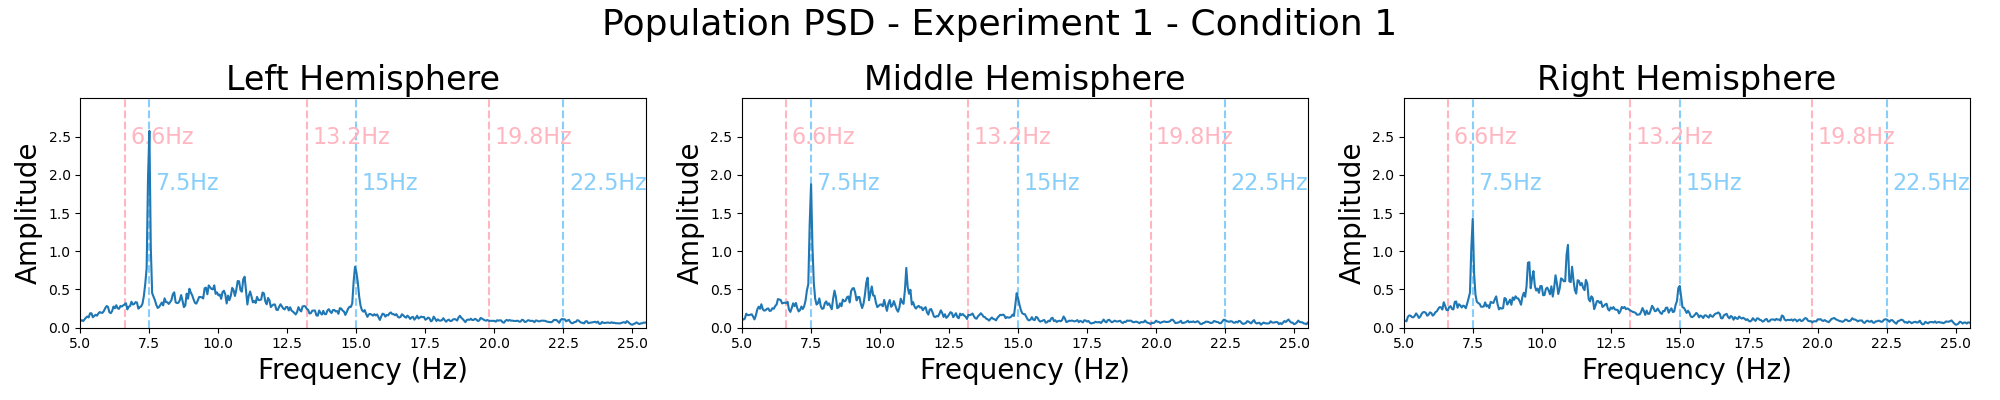
\includegraphics[width=\linewidth]{images/results/e100.png}
        \caption{Condition 1: L$f_{1}$R$\varnothing$}
        \label{fig:e100}
    \end{subfigure}
    
    \begin{subfigure}{1.0\textwidth}
        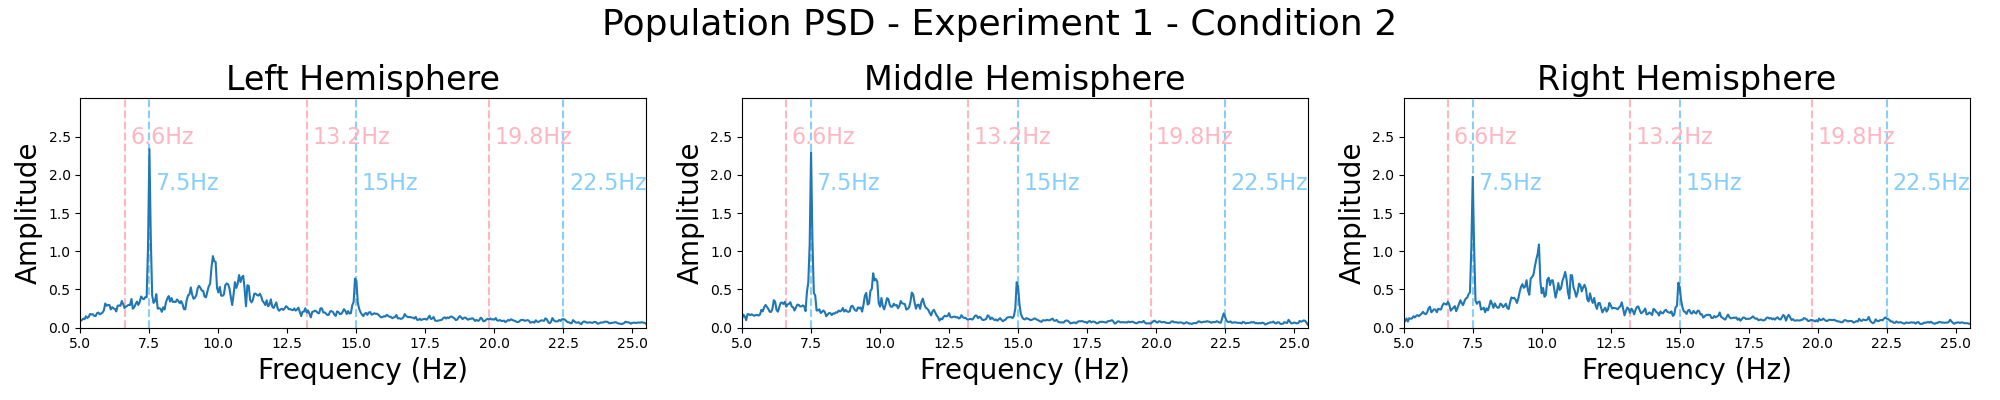
\includegraphics[width=\linewidth]{images/results/e101.png}
        \caption{Condition 2: L$f_{1}$R$f_{1}$}
        \label{fig:e101}
    \end{subfigure}
    
    \begin{subfigure}{1.0\textwidth}
        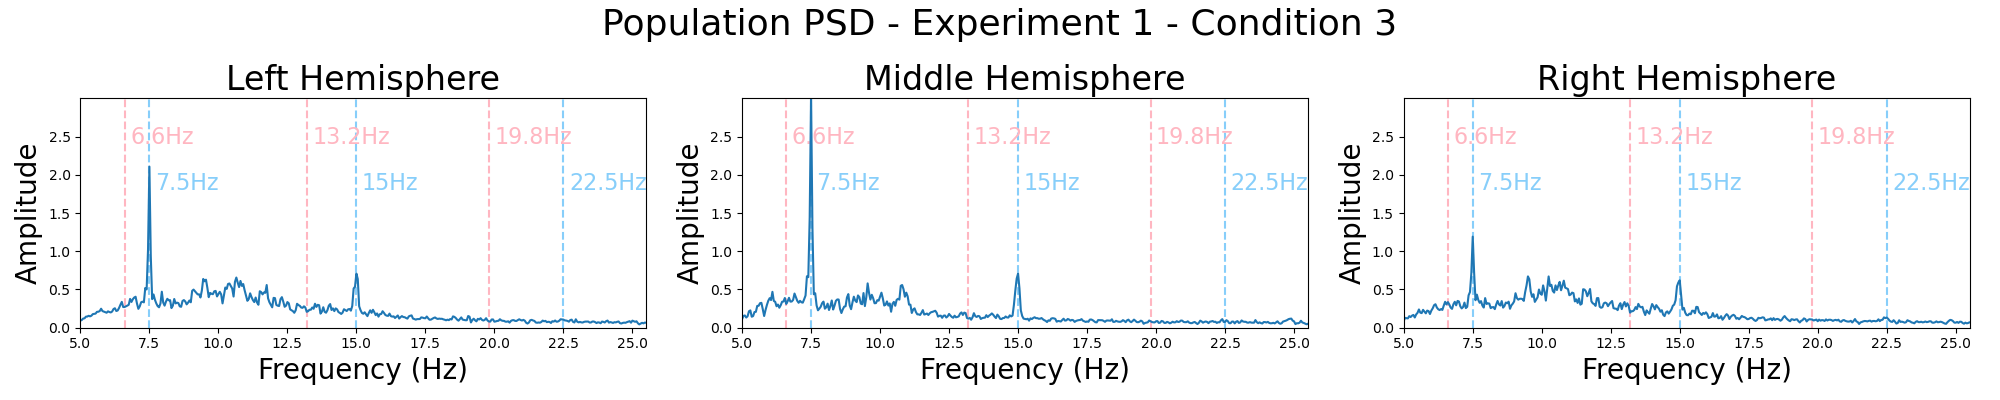
\includegraphics[width=\linewidth]{images/results/e102.png}
        \caption{Condition 3: L$\varnothing$R$f_{1}$}
        \label{fig:e102}
    \end{subfigure}
    \caption{Experiment 1: Population PSD Analysis.}
    \emph{Note: The y-axis is twice the height of the y-axes in the other experiments.}

    \label{fig:e1_population}
\end{figure}







\clearpage


\section{Experiment 2}
\textbf{Conditions:}  L$f_{1}$R$f_{2}$ vs. L$f_{2}$R$f_{2}$  vs. L$f_{2}$R$f_{1}$; ($f_{1}$ = 7.5 Hz, $f_{2}$ = 6.6 Hz)\\ 

\subsection{RQ: Can we differentiate SSVEP responses based on the unique frequency stimuli presented to each eye?}


In Tables \ref{tab:ex2-66}, \ref{tab:ex2-75} the amplitudes of the signals at $f_{2}$ and $f_{1}$ are compared respectively. In table \ref{tab:ex2-ratios} the ratio of the amplitude($f_{1}$)/amplitude($f_{2}$) is calculated per signal and then compared. The statistical comparisons is done using the Wilcoxon method.

We observe low p-values in the cases where one of the compared signals is mono SSVEP (e.g. L$f_{1}$R$f_{1}$ or L$f_{2}$R$f_{2}$). In previous Figures \ref{fig:e1_population} and \ref{fig:e111} it is seen that the amplitude in mono SSVEP is usually double or more that of dual-SSVEP. 

Interesting are the L$f_{1}$R$f_{2}$ vs. L$f_{2}$R$f_{1}$ comparisons in the tables. In Table \ref{tab:ex2-66} the p-values in the lateral PO3, PO4, O2 channels are shown in to be low; in Table \ref{tab:ex2-75} the same is true only for the O1 channel. This shows some, but not strong, evidence against the null hypothesis of \textit{"SSVEP responses cannot be differentiated based on the unique frequency stimuli presented to each eye"}, in the cases where two different frequencies are used.






\begin{table}[ht]
\centering
\begin{tabularx}{\linewidth}{l *{6}{c}}
    \toprule
    \textbf{Compared} & \multicolumn{2}{c}{\textbf{Left}} & \multicolumn{2}{c}{\textbf{Middle}} & \multicolumn{2}{c}{\textbf{Right}} \\
    \textbf{Conditions} & \textbf{p(PO3)} & \textbf{p(O1)} & \textbf{p(POz)} & \textbf{p(Oz)} & \textbf{p(PO4)} & \textbf{p(O2)} \\
    \midrule
    L$f_{1}$R$f_{1}$ vs. L$f_{1}$R$f_{2}$ & <0.01 & <0.01 & 0.03 & <0.01 & 0.21 & <0.01 \\
    L$f_{1}$R$f_{1}$ vs. L$f_{2}$R$f_{2}$ & <0.01 & <0.01 & <0.01 & <0.01 & <0.01 & <0.01 \\
    L$f_{1}$R$f_{1}$ vs. L$f_{2}$R$f_{1}$ & 0.04 & <0.01 & 0.15 & 0.11 & 0.09 & 0.20 \\
    L$f_{1}$R$f_{2}$ vs. L$f_{2}$R$f_{2}$ & <0.01 & 0.14 & 0.03 & <0.01 & <0.01 & <0.01 \\
    L$f_{1}$R$f_{2}$ vs. L$f_{2}$R$f_{1}$ & 0.01 & 0.83 & 0.55 & <0.01 & 0.53 & 0.06 \\
    L$f_{2}$R$f_{2}$ vs. L$f_{2}$R$f_{1}$ & <0.01 & 0.08 & <0.01 & <0.01 & <0.01 & <0.01 \\
    \bottomrule
\end{tabularx}
\caption{Experiment 2: Wilcoxon Test p-values for Amplitudes at 6.6 Hz.}
\label{tab:ex2-66}
\end{table}


\begin{table}[ht]
\centering
\begin{tabularx}{\linewidth}{l *{6}{c}}
    \toprule
    \textbf{Compared} & \multicolumn{2}{c}{\textbf{Left}} & \multicolumn{2}{c}{\textbf{Middle}} & \multicolumn{2}{c}{\textbf{Right}} \\
    \textbf{Conditions} & \textbf{p(PO3)} & \textbf{p(O1)} & \textbf{p(POz)} & \textbf{p(Oz)} & \textbf{p(PO4)} & \textbf{p(O2)} \\
    \midrule
    L$f_{1}$R$f_{1}$ vs. L$f_{1}$R$f_{2}$ & <0.01 & <0.01 & <0.01 & <0.01 & <0.01 & <0.01 \\
    L$f_{1}$R$f_{1}$ vs. L$f_{2}$R$f_{2}$ & <0.01 & <0.01 & <0.01 & <0.01 & <0.01 & <0.01 \\
    L$f_{1}$R$f_{1}$ vs. L$f_{2}$R$f_{1}$ & <0.01 & <0.01 & <0.01 & <0.01 & <0.01 & <0.01 \\
    L$f_{1}$R$f_{2}$ vs. L$f_{2}$R$f_{2}$ & <0.01 & <0.01 & 0.08 & <0.01 & <0.01 & <0.01 \\
    L$f_{1}$R$f_{2}$ vs. L$f_{2}$R$f_{1}$ & 0.28 & 0.01 & 0.85 & 0.19 & 0.16 & 0.24 \\
    L$f_{2}$R$f_{2}$ vs. L$f_{2}$R$f_{1}$ & 0.01 & 0.17 & 0.07 & <0.01 & 0.01 & 0.03 \\
    \bottomrule
\end{tabularx}
\caption{Experiment 2: Wilcoxon Test p-values for Amplitudes at 7.5 Hz.}
\label{tab:ex2-75}
\end{table}



\begin{table}[ht]
\centering
\begin{tabularx}{\linewidth}{l *{6}{c}}
    \toprule
    \textbf{Compared} & \multicolumn{2}{c}{\textbf{Left}} & \multicolumn{2}{c}{\textbf{Middle}} & \multicolumn{2}{c}{\textbf{Right}} \\
    \textbf{Conditions} & \textbf{p(PO3)} & \textbf{p(O1)} & \textbf{p(POz)} & \textbf{p(Oz)} & \textbf{p(PO4)} & \textbf{p(O2)} \\
    \midrule
    L$f_{1}$R$f_{1}$ vs. L$f_{1}$R$f_{2}$ & <0.01 & <0.01 & <0.01 & <0.01 & 0.01 & <0.01 \\
    L$f_{1}$R$f_{1}$ vs. L$f_{2}$R$f_{2}$ & <0.01 & <0.01 & <0.01 & <0.01 & <0.01 & <0.01 \\
    L$f_{1}$R$f_{1}$ vs. L$f_{2}$R$f_{1}$ & <0.01 & <0.01 & <0.01 & <0.01 & <0.01 & <0.01 \\
    L$f_{1}$R$f_{2}$ vs. L$f_{2}$R$f_{2}$ & <0.01 & <0.01 & 0.01 & <0.01 & <0.01 & <0.01 \\
    L$f_{1}$R$f_{2}$ vs. L$f_{2}$R$f_{1}$ & 0.75 & 0.21 & 0.81 & <0.01 & 0.19 & 0.90 \\
    L$f_{2}$R$f_{2}$ vs. L$f_{2}$R$f_{1}$ & <0.01 & 0.01 & <0.01 & <0.01 & <0.01 & <0.01 \\
    \bottomrule
\end{tabularx}
\caption{Experiment 2: Wilcoxon Test p-values for ratio of Amplitudes 6.6 Hz / 7.5 Hz.}
\label{tab:ex2-ratios}
\end{table}


\subsection{RQ: Can we simultaneously elicit separate SSVEP responses in both hemispheres?}
% Separate SSVEP responses cannot be simultaneously elicited in both hemispheres. \\


In the Population PSD Figure \ref{fig:e2_population}, distinct amplitude peaks are observable for the dual stimulating frequencies, 7.5 Hz and 6.6 Hz, indicating the presence of dual-SSVEP responses.

For the specific frequencies, where $f_{1}$ is 7.5 Hz and $f_{2}$ is 6.6 Hz, the patterns in amplitude responses are notable in different conditions as shown in the following figures:

In Figure \ref{fig:e110} (L$f_{1}$R$f_{2}$), it's evident that generally, the amplitude of the 6.6 Hz frequency is lower than that of 7.5 Hz in both the left and right hemispheres. Notably, in the left hemisphere, the amplitude of 6.6 Hz is higher than that in the right hemisphere, which is consistent with the simulation being presented to the right eye.

Moving to Figure \ref{fig:e111} (L$f_{2}$R$f_{2}$), during mono SSVEP stimulation, the 6.6 Hz frequency exhibits a considerably higher SSVEP response, being twice as high as other frequencies. This trend echoes that observed in Figure \ref{fig:e1_population}.

Lastly, Figure \ref{fig:e112} (L$f_{2}$R$f_{1}$) reveals that the amplitude of 6.6 Hz is higher than that of 7.5 Hz in both the left and right hemispheres. However, at 7.5 Hz, the amplitude is higher in the right hemisphere compared to the left. Notably, the amplitude of 6.6 Hz is greater in the left hemisphere than in the right, underscoring a frequency-specific asymmetry.


\begin{figure}[h]
    \centering
    
    \begin{subfigure}{1.0\textwidth}
        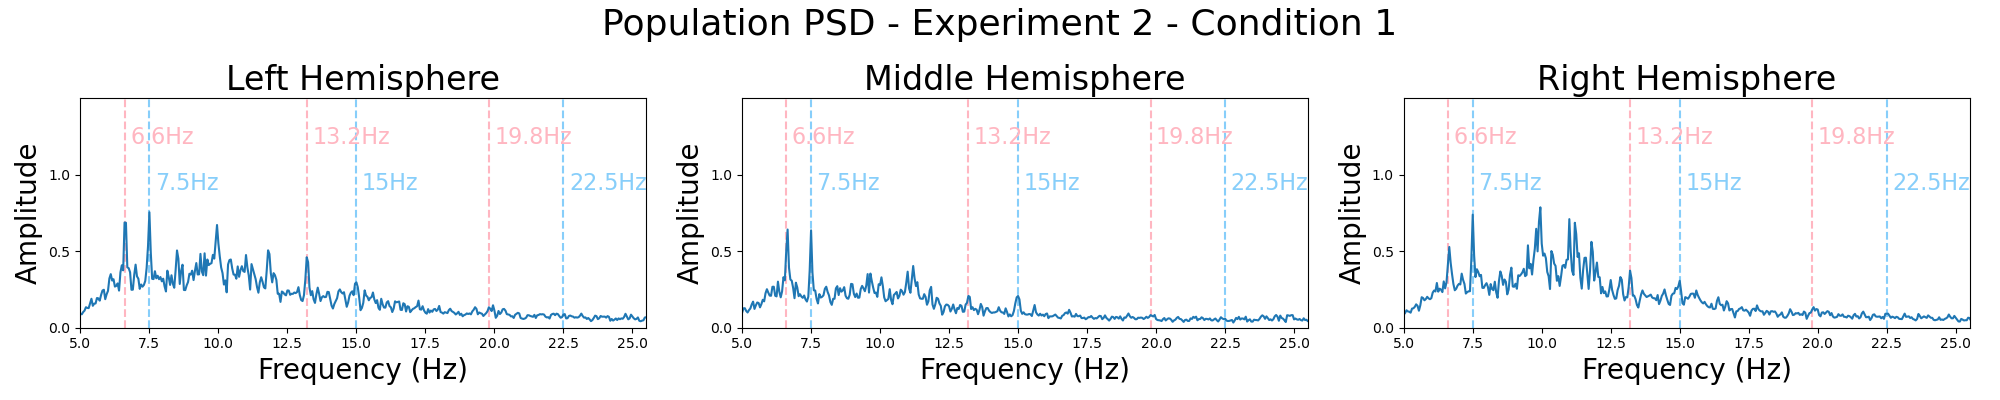
\includegraphics[width=\linewidth]{images/results/e110.png}
        \caption{Condition 1: L$f_{1}$R$f_{2}$}
        \label{fig:e110}
    \end{subfigure}
    

    \begin{subfigure}{1.0\textwidth}
        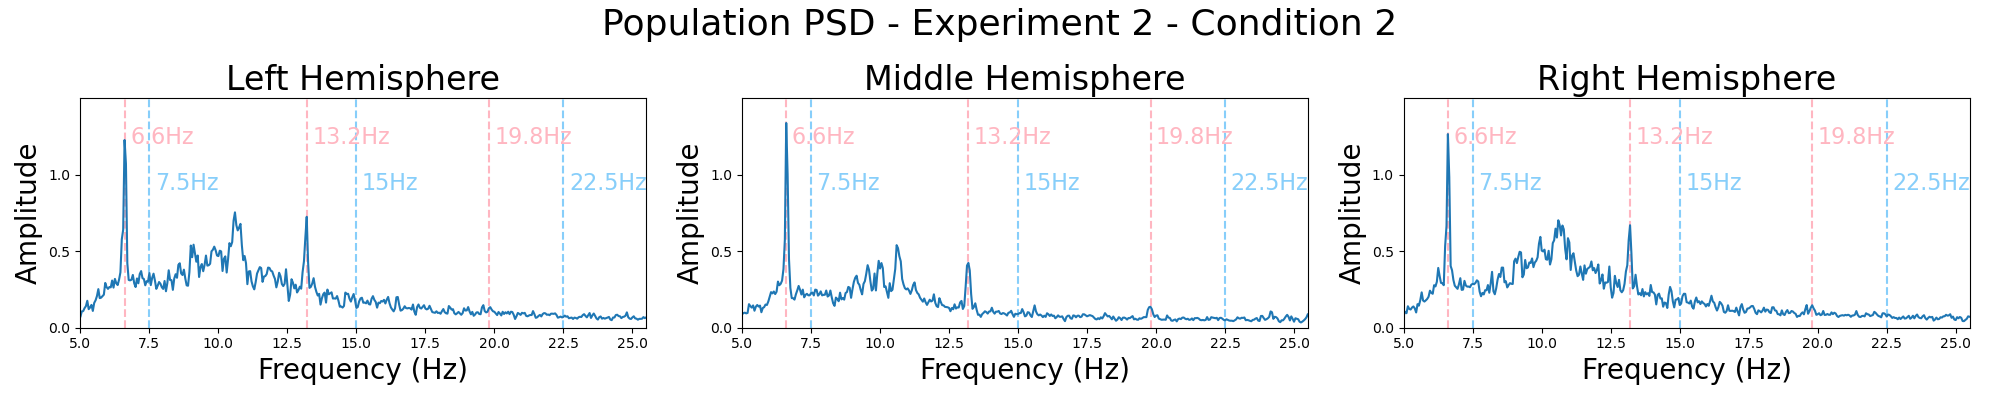
\includegraphics[width=\linewidth]{images/results/e111.png}
        \caption{Condition 2: L$f_{2}$R$f_{2}$}
        \label{fig:e111}
    \end{subfigure}
    
    \begin{subfigure}{1.0\textwidth}
        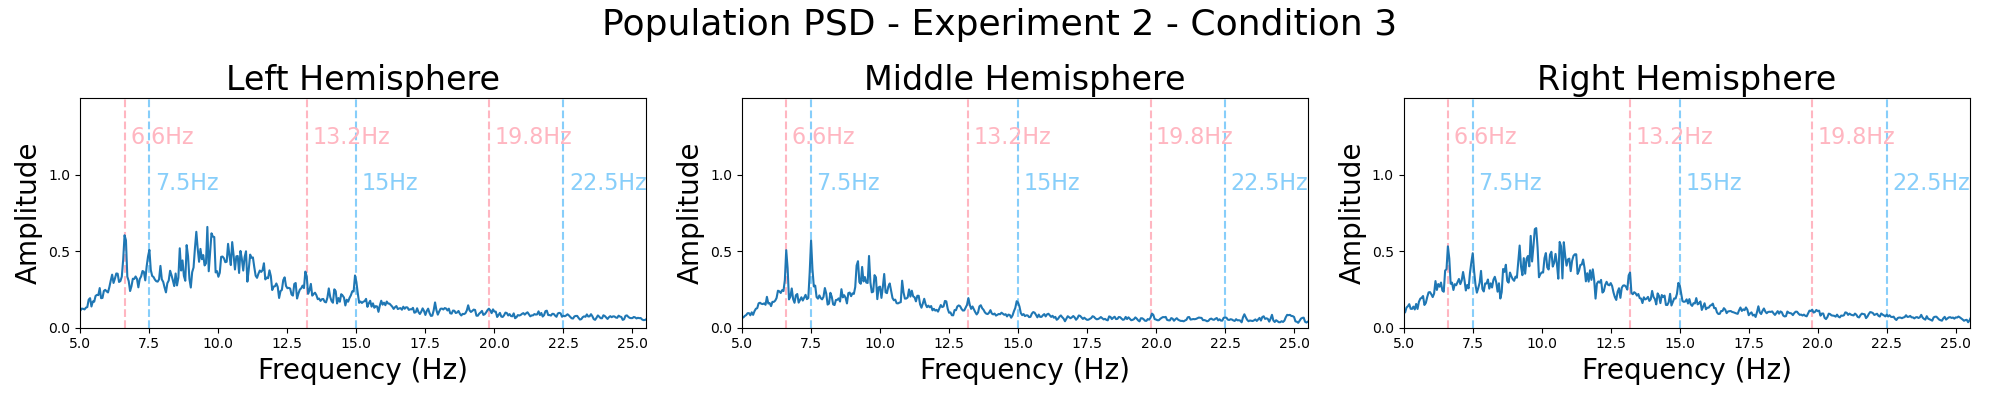
\includegraphics[width=\linewidth]{images/results/e112.png}
        \caption{Condition 3: L$f_{2}$R$f_{1}$}
        \label{fig:e112}
    \end{subfigure}
    
    \caption{Experiment 2: Population PSD Analysis}
    \label{fig:e2_population}
\end{figure}


\clearpage
\section{Experiment 3}
\textbf{Conditions:} BR-L$f_{2}$R$f_{1}$ \\

The experiment aimed to determine whether binocular rivalry could be achieved in a virtual reality environment. All participating individuals consistently reported experiencing binocular rivalry during the course of the experiment.

\begin{figure}[h]
    \centering
    
    \begin{subfigure}{1.0\textwidth}
        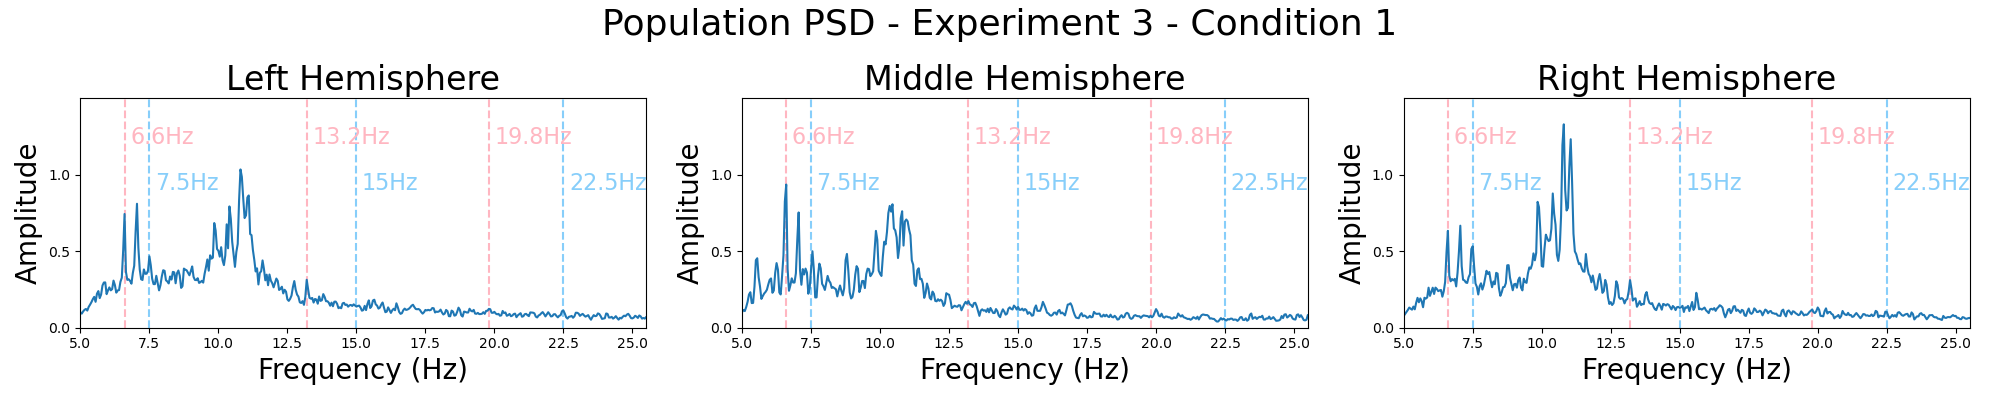
\includegraphics[width=\linewidth]{images/results/e120.png}
        \caption{Condition 1: BR L$f_{2}$,~R$f_{1}$ (BR)}
        \label{fig:e120}
    \end{subfigure}
    \caption{Experiment 3: Population PSD Analysis}
    \label{fig:e3_population}
\end{figure}

While not originally a part of our research questions, we conducted a statistical t-test on the signals to assess hemisphere separation.

The EEG signal underwent segmentation into left, middle, and right hemispheres, and signal strengths at 6.6 Hz and 7.5 Hz were measured. Their ratio was calculated and subjected to testing.

The outcomes of our statistical evaluation are noteworthy. The p-value for the comparison between the Left and Middle hemispheres yielded a relatively high value of 0.915, indicating a lack of substantial difference between these regions. Comparably, the p-value for the Left vs. Right comparison was 0.061, implying a possible discrepancy in strengths. This trend persisted in the Middle vs. Right comparison with a p-value of 0.055.

Although these p-values hover around the conventional significance threshold of 0.05, they do not provide conclusive evidence to reject the null hypothesis, which posits no hemisphere separation.

Of particular interest is the distinct peak observed around 7 Hz in the Population PSD Figure \ref{fig:e3_population}. Remarkably, this distinctive feature was absent in other experimental conditions. Moreover, we noted a heightened presence of noise in the alpha wave range (8–12 Hz).

\begin{table}[h]
\centering
\begin{tabular}{c *{3}{>{\centering\arraybackslash}m{2cm}}}
\toprule
\textbf{Hemisphere Comparison} & \textbf{p-value} \\
\midrule
Left vs. Middle & 0.915 \\
Left vs. Right & 0.061 \\
Middle vs. Right & 0.055 \\
\bottomrule
\end{tabular}
\caption{Experiment 3: T-Test Analysis of p-values for Different Hemispheres.}
\label{tab:pvalues}
\end{table}






\clearpage
\section{Experiment 4}
\textbf{Conditions:} FL-BR-L$f_{2}$R$f_{1}$ vs.  FR-BR-L$f_{2}$R$f_{1}$ \\


\subsection{RQ: Can the direction of participants' attention control or influence binocular rivalry?}

Figure \ref{fig:e4_population} illustrates the Population PSD. A distinct disparity becomes apparent when comparing two scenarios: in the "Focus Right" condition (Figure \ref{fig:e131}), a prominent peak at 7.5 Hz is observable in both hemispheres, accompanied by attenuation of the 6.6 Hz frequency. This stands in contrast to the "Focus Left" scenario (Figure \ref{fig:e130}). These findings present compelling indications that binocular rivalry might be controllable.

The analysis of Tables \ref{tab:ex4-p66}, \ref{tab:ex4-p75}, and \ref{tab:ex4-p66/75} reveals notable statistical distinctions primarily within the PO3, POz, Oz, and O2 channels. However, these differences do not reach a level of statistical significance to refute the null hypothesis.

\begin{figure}[b]
    \centering
    
    \begin{subfigure}{1.0\textwidth}
        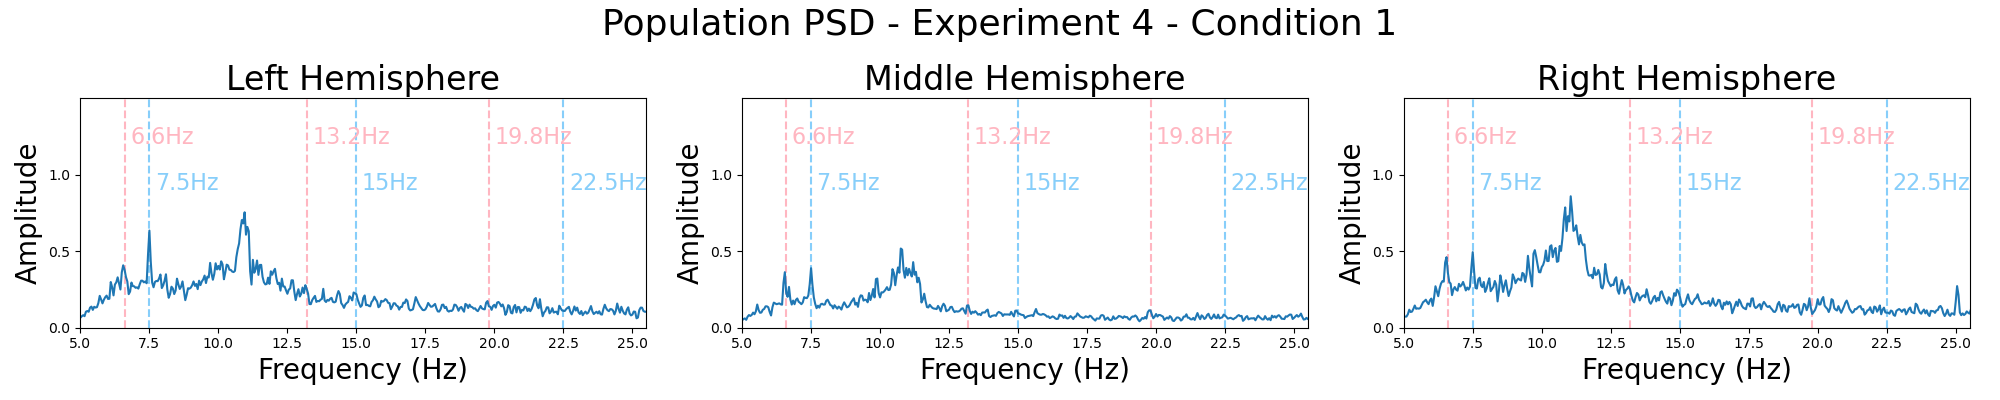
\includegraphics[width=\linewidth]{images/results/e130.png}
        \caption{Condition 1: Focus Left - BR L$f_{2}$,~R$f_{1}$ (FL-BR)}
        \label{fig:e130}
    \end{subfigure}
    
    \begin{subfigure}{1.0\textwidth}
        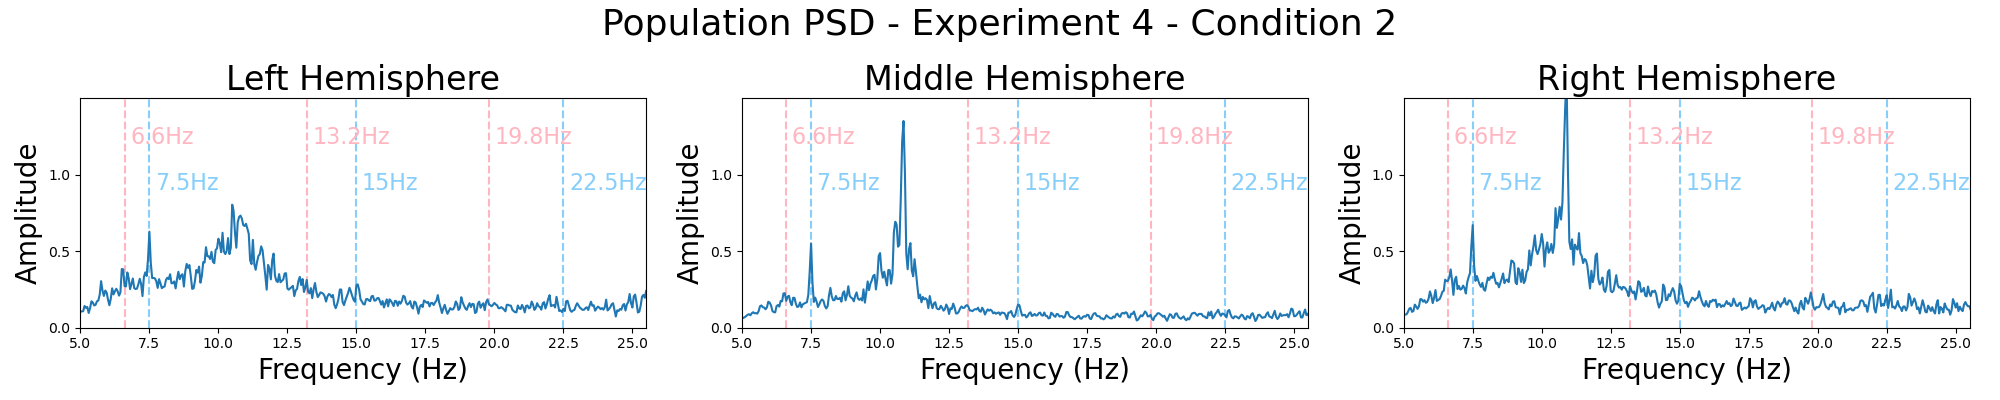
\includegraphics[width=\linewidth]{images/results/e131.png}
        \caption{Condition 2: Focus Right - BR L$f_{2}$,~R$f_{1}$ (FR-BR)}
        \label{fig:e131}
    \end{subfigure}
    
    \caption{Experiment 4: Population PSD Analysis}
    \label{fig:e4_population}
\end{figure}




\begin{table}[b]
\centering
\begin{tabularx}{\linewidth}{l *{6}{c}}
    \toprule
    \textbf{Comparison} & \multicolumn{2}{c}{\textbf{Left}} & \multicolumn{2}{c}{\textbf{Middle}} & \multicolumn{2}{c}{\textbf{Right}} \\
     \textbf{Conditions}& \textbf{p(PO3)} & \textbf{p(O1)} & \textbf{p(POz)} & \textbf{p(Oz)} & \textbf{p(PO4)} & \textbf{p(O2)} \\
    \midrule
    BR vs. FL-BR & 0.03 & 0.97 & 0.45 & 0.27 & 0.88 & 0.22 \\
    BR vs. FR-BR & 0.01 & 0.98 & 0.13 & <0.01 & 0.21 & 0.40 \\
    FL-BR vs. FR-BR & 0.48 & 0.64 & 0.41 & 0.06 & 0.44 & 0.14 \\
    \bottomrule
\end{tabularx}
\caption{Experiment 4: Wilcoxon Test p-values for ratio of Amplitudes 6.6 Hz / 7.5 Hz.}
\label{tab:ex4-p66/75}
\end{table}


\begin{table}[t]
\centering
\begin{tabularx}{\linewidth}{l *{6}{c}}
    \toprule
    \textbf{Comparison} & \multicolumn{2}{c}{\textbf{Left}} & \multicolumn{2}{c}{\textbf{Middle}} & \multicolumn{2}{c}{\textbf{Right}} \\
    \textbf{Conditions} & \textbf{p(PO3)} & \textbf{p(O1)} & \textbf{p(POz)} & \textbf{p(Oz)} & \textbf{p(PO4)} & \textbf{p(O2)} \\
    \midrule
    BR vs. FL-BR & 0.06 & 0.28 & 0.07 & 0.02 & 0.71 & 0.20 \\
    BR vs. FR-BR & 0.02 & 0.63 & 0.64 & <0.01 & 0.03 & 0.18 \\
    FL-BR vs. FR-BR & 0.77 & 0.37 & 0.24 & 0.16 & 0.04 & 0.91 \\
    \bottomrule
\end{tabularx}
\caption{Experiment 4: Wilcoxon Test p-values for Amplitudes at 7.5 Hz.}
\label{tab:ex4-p75}
\end{table}


\begin{table}[t]
\centering
\begin{tabularx}{\linewidth}{l *{6}{c}}
    \toprule
    \textbf{Comparison } & \multicolumn{2}{c}{\textbf{Left}} & \multicolumn{2}{c}{\textbf{Middle}} & \multicolumn{2}{c}{\textbf{Right}} \\
    \textbf{Conditions}& \textbf{p(PO3)} & \textbf{p(O1)} & \textbf{p(POz)} & \textbf{p(Oz)} & \textbf{p(PO4)} & \textbf{p(O2)} \\
    \midrule
    BR vs. FL-BR & 0.65 & 0.23 & 0.05 & 0.40 & 0.88 & 0.47 \\
    BR vs. FR-BR & 0.04 & 0.10 & <0.01 & 0.04 & 0.83 & 0.07 \\
    FL-BR vs. FR-BR & 0.06 & 0.91 & 0.19 & 0.11 & 0.99 & 0.01 \\
    \bottomrule
\end{tabularx}
\caption{Experiment 4: Wilcoxon Test p-values for Amplitudes at 6.6 Hz.}
\label{tab:ex4-p66}
\end{table}

\chapter{Discussion}\label{cha:discussion}

\section{Discussion}

\subsection{Differentiation of Hemisphere-Specific SSVEP Responses Based on the Visually Stimulated Eye}

The research question probed the feasibility of differentiating hemisphere-specific SSVEP responses contingent on the eye subjected to visual stimulation. The null hypothesis posited that no such differentiation exists.

\subsubsection{Methodological Considerations}

To evaluate the observed differences, a significance level of \( \alpha = 0.05 \) was employed. Given the non-Gaussian distribution of the PSD, non-parametric tests were favored over traditional parametric tests. Specifically, the Wilcoxon signed-rank test was utilized, which is particularly apt for data that deviate from a normal distribution.

\subsubsection{Electrode-Specific Findings}

\paragraph{Central Channels: POz and Oz}
In alignment with expectations, the null hypothesis was predominantly upheld for the central channels, with the exception of the Oz channel under the third condition. This outcome is not entirely surprising given the central location of the POz and Oz electrodes, which are positioned in a region close to both hemispheres. As such, they are likely to capture a blend of neural activity from both sides, potentially diluting the hemisphere-specific responses that might have been observed with more laterally placed electrodes.

\paragraph{Lateral Channels: PO3, O1, and O2}
The lateral channels, particularly PO3 and O1, showed distinct patterns across the three conditions. In the first condition, comparing the left eye being stimulated versus both eyes, and in the second condition, comparing the left eye versus the right eye, both channels provided strong evidence against the null hypothesis. These findings are consistent with contralateral processing theory, as these channels are situated in the left hemisphere and primarily process input from the right eye.

In the third condition, where both eyes were compared to the right eye, the null hypothesis was not rejected for the PO3 and O1 channels. This outcome is primarily a reflection of the EEG device's limited spatial resolution. While these channels are located in the left hemisphere and process input from the right eye, the device's limitations make it challenging to distinguish between the right eye being stimulated and both eyes being stimulated.

For the O2 channel, the null hypothesis was not rejected when comparing the left eye being stimulated versus both eyes. This outcome is primarily attributed to the limited spatial resolution of the EEG device. The O2 channel, situated in the right hemisphere, processes input from the left eye. However, the device's limitations make it challenging to distinguish between the left eye being stimulated and both eyes being stimulated.

\paragraph{Anomalous Findings: PO4 Channel}
The PO4 channel presented an unexpected pattern, especially when compared to its counterpart, PO3. This discrepancy could be attributed to multiple factors, including the limited spatial resolution of the EEG device and the potential influence of eye dominance, a less explored but potentially significant variable.

\subsubsection{Population PSD Analysis}
Population Power Spectral Density (PSD) was analyzed across three regions: left (PO3, O1), middle (POz, Oz), and right (PO4, O2), as depicted in Figure~\ref{fig:e1_population}. The amplitude values across different conditions offered varying degrees of support for the research question. Some conditions contradicted established theories of contralateral processing, while others reinforced them.

\paragraph{First Condition: Contradictory Findings}
The amplitude values in the first condition contradicted both the research question and the established understanding of contralateral processing. A speculative explanation could be the influence of peripheral vision stimuli on SSVEP responses, although this hypothesis currently lacks empirical support.

\paragraph{Second Condition: Dominant Eye Effect}
The second condition revealed amplitude values that align with the notion of a dominant right eye, as evidenced by higher amplitude in the left hemisphere. This finding further substantiates the theory of contralateral processing.

\paragraph{Third Condition: Support for Research Question}
The third condition provided evidence in favor of the research question, demonstrating a higher amplitude in the left hemisphere when the right eye was stimulated. The elevated amplitude in the middle region could be attributed to a combination of eye dominance and the limitations of the EEG device.



\section{Experiment 2}

\subsection{Research Question 1: Differentiation of SSVEP Responses Based on Unique Frequency Stimuli}

The first research question aimed to differentiate SSVEP responses based on the unique frequency stimuli presented to each eye. The p-values from Tables \ref{tab:ex2-66}, \ref{tab:ex2-75}, and \ref{tab:ex2-ratios} already indicated a nuanced ability to differentiate these responses, especially in the left and middle regions. This evidence is further supported by the Population PSD Figure \ref{fig:e2_population}, which shows distinct amplitude peaks for both stimulating frequencies, 6.6 Hz and 7.5 Hz.

\subsection{Research Question 2: Simultaneous Elicitation of Separate SSVEP Responses}

\paragraph{First Trial}
Both unique frequencies (6.6 Hz and 7.5 Hz) elicited distinct SSVEP responses in both hemispheres. The p-values had already indicated that the amplitude for the 7.5 Hz frequency was higher in both hemispheres, contradicting the dominant eye theory. The absence of IM components highlights the advantages of using VR to control stimuli for each eye separately. The Population PSD Figure \ref{fig:e2_population} further supports this.

\paragraph{Second Trial}
The p-values showed a clear peak at 6.6 Hz across all regions, reinforcing the feasibility of a dual-SSVEP paradigm in VR. This is further supported by the Population PSD Figure \ref{fig:e2_population}.

\paragraph{Third Trial}
The p-values indicated that the amplitude of the 6.6 Hz frequency was higher than that of the 7.5 Hz. This is further supported by the Population PSD Figure \ref{fig:e2_population}, and the reason for this phenomenon remains unclear but warrants further investigation.

\paragraph{Amplitude Observations}
The Population PSD Figure \ref{fig:e2_population} shows distinct amplitude peaks for both stimulating frequencies, 7.5 Hz and 6.6 Hz, further substantiating the p-value evidence that dual-SSVEP has been achieved in a virtual reality environment.

\paragraph{Presence of Dual-SSVEP}
The p-values and the presence of well-defined amplitude peaks at both stimulating frequencies substantiate the concept of achieving dual-SSVEP responses within the immersive domain of virtual reality.
.

\section{Experiment 4}

\subsubsection{Individual Frequency Comparisons}

\paragraph{7.5 Hz Frequency:} 
The comparison between Experiment 3 and the conditions of Experiment 4 for the 7.5 Hz frequency yielded mixed results. While most channels did not provide sufficient evidence to reject the null hypothesis, channels PO3, Oz, and PO4 showed evidence against it in the comparison with the second condition of Experiment 4.

\paragraph{6.6 Hz Frequency:} 
For the 6.6 Hz frequency, the channels largely supported the null hypothesis, except for PO3, POz, and Oz when comparing Experiment 3 with the second condition of Experiment 4.

\subsubsection{Ratio of Amplitude Frequencies}

The comparison of the amplitude ratios between the 6.6 Hz and 7.5 Hz frequencies predominantly supported the null hypothesis, except for specific channels like PO3 and Oz.

\subsubsection{Overall Interpretation and Practical Implications}

The individual frequency comparisons and the ratio comparisons collectively suggest that the role of directed attention in binocular rivalry is complex and not easily influenced by conscious control. The inconsistencies among channels could either indicate that these channels are more sensitive to changes in attentional focus or reflect the limitations of the EEG device used. These findings underscore the need for further research using more advanced neuroimaging techniques to delve into the complexities of neural processes underlying binocular rivalry.


\chapter{Conclusion}\label{cha:conclusion}

The primary objective of this research was to explore the feasibility of differentiating SSVEP responses based on the eye being visually stimulated. Additionally, the study aimed to investigate the possibility of eliciting separate SSVEP responses in a VR environment. These objectives were set within the broader context of advancing BCI technologies.

The study tackled multiple research questions across different experiments, each contributing to a nuanced understanding of SSVEP responses and their underlying neural mechanisms. Experiment 1 primarily focused on the feasibility of differentiating hemisphere-specific SSVEP responses based on the eye being visually stimulated. While central channels like POz and Oz largely upheld the null hypothesis, suggesting they are not ideal for this differentiation, lateral channels such as PO3, O1, and O2 provided evidence against the null hypothesis, particularly when the left eye was compared to both eyes or the right eye. This lends partial support to the feasibility of differentiating SSVEP responses based on the eye being stimulated. Experiment 2 took this a step further by exploring the ability to elicit separate SSVEP responses in a Virtual Reality (VR) environment using unique frequency stimuli for each eye. The evidence strongly supported this ability. Finally, Experiment 4 added complexity to the picture by investigating the role of directed attention in binocular rivalry. The findings were mixed, suggesting that the role of attention in this phenomenon is influenced by multiple factors, including the limitations of the EEG device used.

The findings suggest that contralateral processing theories hold true for lateral channels, but the central channels' location makes them less reliable for this differentiation. The evidence from Experiment 2 supports the concept of dual-SSVEP in VR, opening up new avenues for BCI applications. However, the complexities observed in Experiment 4 indicate that directed attention and binocular rivalry are influenced by a myriad of factors, including the limitations of the EEG device used.

The study had several limitations, including the spatial resolution of the EEG device, which affected the reliability of the findings. Anomalous results in channels like PO4 also point to potential variables like eye dominance that were not accounted for. Additionally, the study employed non-parametric tests due to the non-Gaussian distribution of the data, which may not be the most robust method for all conditions.

Given the limitations and the complexities observed, future research should consider using more advanced neuroimaging techniques to delve deeper into the neural processes underlying SSVEP responses and binocular rivalry. Studies could also explore the influence of peripheral vision stimuli on SSVEP responses, especially given the contradictory findings observed in the amplitude values during the first condition and the inconsistencies between PO3 and PO4 channels. Further work could also investigate the role of eye dominance in SSVEP responses, which could be a significant variable affecting the results.

In summary, while the study provides valuable insights into the differentiation of SSVEP responses and the feasibility of dual-SSVEP in VR, it also raises several questions that warrant further investigation. The findings have important implications for the development of more sophisticated and reliable BCIs but also underscore the need for continued research in this rapidly evolving field.


% If you have appendices:
% \appendixpage*          
% \appendix
% % \chapter{Table Appendix}
\label{app:T}

\begin{table}[htbp]
  \centering
  \begin{tabularx}{\textwidth}{cccc}
      \hline     
      {\textbf{P.}} & {\textbf{SNR - L$f_{1}$,~R$\varnothing$}} & \textbf{SNR - L$\varnothing$,~R$f_{1}$} & \multicolumn{1}{c}{\textbf{p-value}}\\
      \hline
      1 & 0.80, 0.27, 0.50, 0.38, 0.73, 0.24 & 0.58, 0.24, 0.36, 0.27, 0.57, 0.29 &  0.09 \\
      1 & 0.56, 0.20, 0.41, 0.32, 0.37, 0.22 & 0.54, 0.25, 0.31, 0.24, 0.66, 0.28 &  1.0 \\
      2 & 0.38, 0.31, 0.31, 0.37, 0.45, 0.43 & 0.36, 0.30, 0.42, 0.40, 0.46, 0.36 &  0.84 \\
      2 & 0.47, 0.39, 0.34, 0.31, 0.50, 0.48 & 0.39, 0.34, 0.44, 0.31, 0.51, 0.35 &  0.69 \\
      3 & 0.41, 0.32, 0.30, 0.38, 0.37, 0.39 & 0.31, 0.28, 0.27, 0.32, 0.30, 0.34 &  0.03 \\
      4 & 0.38, 0.40, 0.36, 0.37, 0.40, 0.28 & 0.36, 0.40, 0.39, 0.33, 0.39, 0.33 &  1.0 \\
      5 & 0.37, 0.26, 0.41, 0.50, 0.21, 0.40 & 0.35, 0.35, 0.38, 0.37, 0.25, 0.38 &  0.84 \\
      5 & 0.39, 0.33, 0.41, 0.45, 0.36, 0.38 & 0.32, 0.39, 0.37, 0.38, 0.37, 0.35 &  0.44 \\
      6 & 0.59, 0.56, 0.34, 0.36, 0.71, 0.46 & 0.47, 0.60, 0.34, 0.38, 0.52, 0.45 &  0.56 \\
      7 & 0.34, 0.32, 0.28, 0.27, 0.29, 0.38 & 0.36, 0.33, 0.34, 0.32, 0.30, 0.29 &  0.44 \\
      8 & 0.43, 0.27, 0.34, 0.33, 0.38, 0.23 & 0.29, 0.23, 0.30, 0.28, 0.43, 0.25 &  0.31 \\
      all & 0.30, 0.18, 0.24, 0.24, 0.22, 0.21 & 0.28, 0.21, 0.24, 0.21, 0.24, 0.23 & 0.56 \\
      \hline
  \end{tabularx}
  \caption{Comparison of SNR between L$f_{7.5 Hz}$,~R$\varnothing$ and L$\varnothing$,~R$f_{7.5 Hz}$}
  \emph{Can we differentiate SSVEP responses based on which eye was stimulated?}
  \label{tab:rq1c1}
\end{table}

\begin{table}[htbp]
  \centering
  \begin{tabularx}{\textwidth}{cccc}
      \hline      
      {\textbf{P.}} & {\textbf{SNR - L$f_{1}$,~R$\varnothing$}} & \textbf{SNR - L$f_{1}$,~R$f_{1}$} & \multicolumn{1}{c}{\textbf{p-value}}\\
      \hline
      1 & 0.50, 0.18, 0.35, 0.27, 0.42, 0.19 & 0.34, 0.16, 0.27, 0.23, 0.27, 0.19 &  0.03 \\
1 & 0.34, 0.13, 0.28, 0.22, 0.23, 0.16 & 0.32, 0.16, 0.24, 0.18, 0.26, 0.18 &  0.84 \\
2 & 0.21, 0.18, 0.18, 0.21, 0.25, 0.24 & 0.25, 0.20, 0.21, 0.22, 0.36, 0.31 &  0.03 \\
2 & 0.24, 0.20, 0.19, 0.18, 0.27, 0.26 & 0.25, 0.17, 0.21, 0.20, 0.36, 0.27 &  0.31 \\
3 & 0.24, 0.20, 0.20, 0.23, 0.22, 0.23 & 0.22, 0.19, 0.19, 0.22, 0.20, 0.22 &  0.03 \\
4 & 0.22, 0.23, 0.22, 0.23, 0.22, 0.19 & 0.18, 0.22, 0.21, 0.19, 0.24, 0.21 &  0.56 \\
5 & 0.23, 0.18, 0.27, 0.28, 0.18, 0.24 & 0.19, 0.19, 0.29, 0.27, 0.19, 0.21 &  0.84 \\
5 & 0.23, 0.20, 0.26, 0.28, 0.25, 0.22 & 0.23, 0.21, 0.28, 0.24, 0.25, 0.23 &  0.84 \\
6 & 0.31, 0.29, 0.23, 0.22, 0.36, 0.27 & 0.33, 0.29, 0.24, 0.20, 0.41, 0.30 &  0.31 \\
7 & 0.24, 0.18, 0.20, 0.18, 0.17, 0.26 & 0.20, 0.19, 0.19, 0.17, 0.14, 0.26 &  0.31 \\
8 & 0.23, 0.17, 0.20, 0.21, 0.21, 0.15 & 0.17, 0.13, 0.19, 0.18, 0.20, 0.17 &  0.09 \\
all & 0.30, 0.18, 0.24, 0.24, 0.22, 0.21 & 0.27, 0.19, 0.22, 0.23, 0.22, 0.22 & 0.44 \\
   \hline
  \end{tabularx}
  \caption{Comparison of SNR between L$f_{7.5 Hz}$,~R$\varnothing$ and L$f_{7.5 Hz}$,~R$f_{7.5 Hz}$}
  \emph{Can we differentiate SSVEP responses based on which eye was stimulated?}
  \label{tab:rq1c2}
\end{table}

\begin{table}[htbp]
  \centering
  \begin{tabularx}{\textwidth}{cccc}
      \hline      
      {\textbf{P.}} & {\textbf{SNR - L$\varnothing$,~R$f_{1}$}} & \textbf{SNR - L$f_{1}$,~R$f_{1}$} & \multicolumn{1}{c}{\textbf{p-value}}\\
      \hline
      1 & 0.34, 0.16, 0.27, 0.23, 0.27, 0.19 & 0.37, 0.16, 0.24, 0.20, 0.35, 0.22 &  0.69 \\
1 & 0.32, 0.16, 0.24, 0.18, 0.26, 0.18 & 0.35, 0.17, 0.21, 0.17, 0.38, 0.20 &  0.44 \\
2 & 0.25, 0.20, 0.21, 0.22, 0.36, 0.31 & 0.20, 0.17, 0.23, 0.20, 0.27, 0.21 &  0.09 \\
2 & 0.25, 0.17, 0.21, 0.20, 0.36, 0.27 & 0.20, 0.18, 0.25, 0.18, 0.29, 0.19 &  0.22 \\
3 & 0.22, 0.19, 0.19, 0.22, 0.20, 0.22 & 0.20, 0.18, 0.19, 0.23, 0.19, 0.22 &  0.31 \\
4 & 0.18, 0.22, 0.21, 0.19, 0.24, 0.21 & 0.21, 0.23, 0.23, 0.21, 0.22, 0.21 &  0.44 \\
5 & 0.19, 0.19, 0.29, 0.27, 0.19, 0.21 & 0.23, 0.23, 0.27, 0.25, 0.19, 0.24 &  0.31 \\
5 & 0.23, 0.21, 0.28, 0.24, 0.25, 0.23 & 0.21, 0.24, 0.26, 0.25, 0.25, 0.23 &  0.84 \\
6 & 0.33, 0.29, 0.24, 0.20, 0.41, 0.30 & 0.27, 0.31, 0.23, 0.23, 0.29, 0.26 &  0.31 \\
7 & 0.20, 0.19, 0.19, 0.17, 0.14, 0.26 & 0.22, 0.20, 0.25, 0.22, 0.16, 0.19 &  0.44 \\
8 & 0.17, 0.13, 0.19, 0.18, 0.20, 0.17 & 0.18, 0.14, 0.18, 0.17, 0.24, 0.17 &  0.56 \\
all & 0.27, 0.19, 0.22, 0.23, 0.22, 0.22 & 0.28, 0.21, 0.24, 0.21, 0.24, 0.23 & 0.16 \\
   \hline
  \end{tabularx}
  \caption{Comparison of SNR between L$\varnothing$,~R$f_{7.5 Hz}$ and L$f_{7.5 Hz}$,~R$f_{7.5 Hz}$}
  \emph{Can we differentiate SSVEP responses based on which eye was stimulated?}
  \label{tab:rq1c3}
\end{table}


\begin{table}[htbp]
  \centering
  \begin{tabularx}{\textwidth}{cCCc}
      \hline      
      {\textbf{P.}} & \textbf{SNR - Stimulated} & \textbf{SNR - Not Stimulated} & \multicolumn{1}{c}{\textbf{p-value}}\\
      \hline
      1 & 0.35, 0.19, 0.37, 0.20 & 0.50, 0.27, 0.24, 0.22 &  0.62 \\
      1 & 0.28, 0.16, 0.35, 0.17 & 0.34, 0.22, 0.21, 0.20 &  0.88 \\
      2 & 0.18, 0.24, 0.20, 0.20 & 0.21, 0.21, 0.23, 0.21 &  0.38 \\
      2 & 0.19, 0.26, 0.20, 0.18 & 0.24, 0.18, 0.25, 0.19 &  0.88 \\
      3 & 0.20, 0.23, 0.20, 0.23 & 0.24, 0.23, 0.19, 0.22 &  0.88 \\
      4 & 0.22, 0.19, 0.21, 0.21 & 0.22, 0.23, 0.23, 0.21 &  0.25 \\
      5 & 0.27, 0.24, 0.23, 0.25 & 0.23, 0.28, 0.27, 0.24 &  0.62 \\
      5 & 0.26, 0.22, 0.21, 0.25 & 0.23, 0.28, 0.26, 0.23 &  0.62 \\
      6 & 0.23, 0.27, 0.27, 0.23 & 0.31, 0.22, 0.23, 0.26 &  1.0 \\
      7 & 0.20, 0.26, 0.22, 0.22 & 0.24, 0.18, 0.25, 0.19 &  0.88 \\
      8 & 0.20, 0.15, 0.18, 0.17 & 0.23, 0.21, 0.18, 0.17 &  0.38 \\
      all & 0.24, 0.21, 0.28, 0.21 & 0.30, 0.24, 0.24, 0.23 & 0.62 \\\hline
  \end{tabularx}
  \caption{Comparison of SNR between Stimulated and Not Stimulated (L$f_{7.5 Hz}$,~R$\varnothing$ and L$\varnothing$,~R$f_{7.5 Hz})$}
  \emph{Can we discern which eye saw the stimulation based on hemisphere separation?}
  \label{tab:rq2c1}
\end{table}

\begin{table}[htbp]
    \centering
    \begin{tabularx}{\textwidth}{cCCc}
        \hline      
        {\textbf{P.}} & \textbf{SNR - Stimulated} & \textbf{SNR - Not Stimulated} & \multicolumn{1}{c}{\textbf{p-value}}\\
        \hline
        1 & 0.35, 0.19 & 0.50, 0.27 &  0.5 \\
        1 & 0.28, 0.16 & 0.34, 0.22 &  0.5 \\
        2 & 0.18, 0.24 & 0.21, 0.21 &  1.0 \\
        2 & 0.19, 0.26 & 0.24, 0.18 &  1.0 \\
        3 & 0.20, 0.23 & 0.24, 0.23 &  0.5 \\
        4 & 0.22, 0.19 & 0.22, 0.23 &  0.5 \\
        5 & 0.27, 0.24 & 0.23, 0.28 &  1.0 \\
        5 & 0.26, 0.22 & 0.23, 0.28 &  1.0 \\
        6 & 0.23, 0.27 & 0.31, 0.22 &  1.0 \\
        7 & 0.20, 0.26 & 0.24, 0.18 &  1.0 \\
        8 & 0.20, 0.15 & 0.23, 0.21 &  0.5 \\
        all & 0.24, 0.21 & 0.30, 0.24 & 0.5 \\
        \hline
    \end{tabularx}
    \caption{Comparison of SNR between Stimulated and Not Stimulated (L$f_{7.5 Hz}$,~R$\varnothing$)}
    \emph{Can we discern which eye saw the stimulation based on hemisphere separation?}
    \label{tab:rq2c2}
  \end{table}

  \begin{table}[htbp]
    \centering
    \begin{tabularx}{\textwidth}{cCCc}
        \hline      
        {\textbf{P.}} & \textbf{SNR - Stimulated} & \textbf{SNR - Not Stimulated} & \multicolumn{1}{c}{\textbf{p-value}}\\
        \hline
        1 & 0.37, 0.20 & 0.24, 0.22 &  1.0 \\
        1 & 0.35, 0.17 & 0.21, 0.20 &  1.0 \\
        2 & 0.20, 0.20 & 0.23, 0.21 &  0.5 \\
        2 & 0.20, 0.18 & 0.25, 0.19 &  0.5 \\
        3 & 0.20, 0.23 & 0.19, 0.22 &  0.5 \\
        4 & 0.21, 0.21 & 0.23, 0.21 &  1.0 \\
        5 & 0.23, 0.25 & 0.27, 0.24 &  1.0 \\
        5 & 0.21, 0.25 & 0.26, 0.23 &  1.0 \\
        6 & 0.27, 0.23 & 0.23, 0.26 &  1.0 \\
        7 & 0.22, 0.22 & 0.25, 0.19 &  1.0 \\
        8 & 0.18, 0.17 & 0.18, 0.17 &  1.0 \\
        all & 0.28, 0.21 & 0.24, 0.23 & 1.0 \\
        \hline
    \end{tabularx}
    \caption{Comparison of SNR between Stimulated and Not Stimulated (L$\varnothing$,~R$f_{7.5 Hz}$)}
    \emph{Can we discern which eye saw the stimulation based on hemisphere separation?}
    \label{tab:rq2c3}
  \end{table}


\begin{table}[htbp]
    \centering
    \begin{tabularx}{\textwidth}{cccc}
        \hline      
        {\textbf{P.}} & {\textbf{SNR - L$f_{1}$,~R$f_{2}$}} & \textbf{SNR - L$f_{2}$,~R$f_{1}$} & \multicolumn{1}{c}{\textbf{p-value}}\\
        \hline
        1 & 0.45, 0.22, 0.35, 0.30, 0.36, 0.23 & 0.42, 0.28, 0.31, 0.28, 0.36, 0.27 &  1.0 \\
1 & 0.38, 0.23, 0.34, 0.27, 0.16, 0.22 & 0.44, 0.28, 0.42, 0.32, 0.21, 0.30 &  0.03 \\
2 & 0.35, 0.28, 0.34, 0.33, 0.33, 0.34 & 0.35, 0.31, 0.35, 0.30, 0.36, 0.37 &  0.22 \\
2 & 0.47, 0.29, 0.40, 0.31, 0.37, 0.38 & 0.40, 0.31, 0.36, 0.29, 0.35, 0.35 &  0.16 \\
3 & 0.31, 0.26, 0.29, 0.36, 0.31, 0.30 & 0.28, 0.26, 0.27, 0.28, 0.29, 0.31 &  0.16 \\
4 & 0.34, 0.40, 0.40, 0.28, 0.40, 0.29 & 0.36, 0.37, 0.37, 0.27, 0.35, 0.32 &  0.31 \\
5 & 0.29, 0.30, 0.30, 0.41, 0.17, 0.36 & 0.26, 0.32, 0.29, 0.37, 0.16, 0.34 &  0.22 \\
5 & 0.36, 0.38, 0.35, 0.45, 0.22, 0.42 & 0.31, 0.38, 0.33, 0.36, 0.23, 0.42 &  0.44 \\
6 & 0.45, 0.47, 0.36, 0.35, 0.42, 0.34 & 0.46, 0.44, 0.37, 0.34, 0.38, 0.31 &  0.31 \\
7 & 0.33, 0.38, 0.28, 0.30, 0.32, 0.35 & 0.33, 0.38, 0.27, 0.26, 0.28, 0.36 &  0.44 \\
8 & 0.28, 0.23, 0.29, 0.29, 0.37, 0.21 & 0.30, 0.20, 0.30, 0.25, 0.33, 0.25 &  0.84 \\
all & 0.34, 0.29, 0.33, 0.33, 0.24, 0.29 & 0.37, 0.31, 0.33, 0.30, 0.23, 0.34 & 0.69 \\
     \hline
    \end{tabularx}
    \caption{Comparison of SNR between L$f_{7.5 Hz}$,~R$f_{6.6 Hz}$ and L$f_{6.6 Hz}$,~R$f_{7.5 Hz}$}
    \emph{Can we differentiate SSVEP responses based on the unique frequency stimuli presented to each eye?}
    \label{tab:rq3c1}
  \end{table}  

% \section{Research Question 4: Can we simultaneously elicit separate SSVEP responses in both hemispheres?}

% \chapter{Results Appendix}
\label{app:R}

\begin{figure}[h]
    \centering
    \begin{subfigure}{0.3\textwidth}
        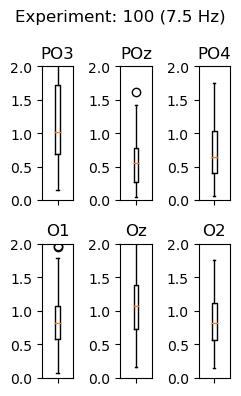
\includegraphics[width=\linewidth]{images/appendix/10075.png}
        \label{fig:10075}
    \end{subfigure}
    \hfill
    \begin{subfigure}{0.3\textwidth}
        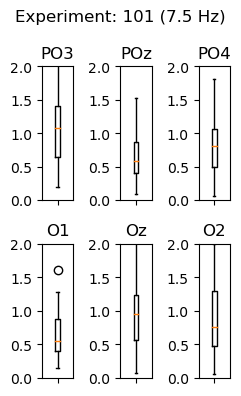
\includegraphics[width=\linewidth]{images/appendix/10175.png}
        \label{fig:10175}
    \end{subfigure}
    \hfill
    \begin{subfigure}{0.3\textwidth}
        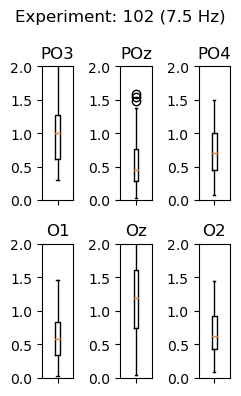
\includegraphics[width=\linewidth]{images/appendix/10275.png}
        \label{fig:10275}
    \end{subfigure}
    \caption{Experiment 1 - Conditions 0, 1, and 2: Boxplots per hemisphere.}
    \label{fig:1-675}
\end{figure}


\begin{figure}[ht]
    \centering
    \begin{subfigure}{0.25\linewidth}
        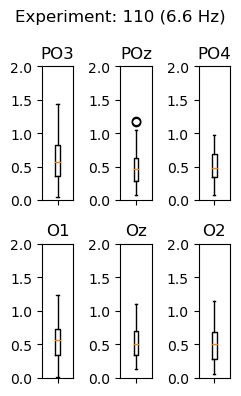
\includegraphics[width=\linewidth]{images/appendix/11066.png}
        \label{fig:11066}
    \end{subfigure}
    \begin{subfigure}{0.25\linewidth}
        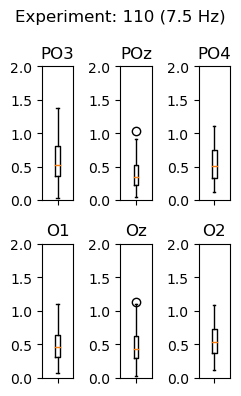
\includegraphics[width=\linewidth]{images/appendix/11075.png}
        \label{fig:11075}
    \end{subfigure}
    
    \begin{subfigure}{0.25\linewidth}
        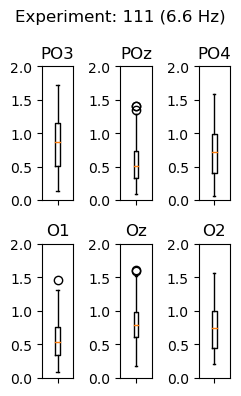
\includegraphics[width=\linewidth]{images/appendix/11166.png}
        \label{fig:11166}
    \end{subfigure}
    \begin{subfigure}{0.25\linewidth}
        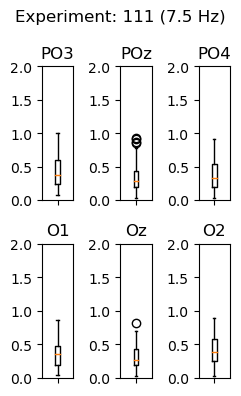
\includegraphics[width=\linewidth]{images/appendix/11175.png}
        \label{fig:11175}
    \end{subfigure}
        
    \begin{subfigure}{0.25\linewidth}
        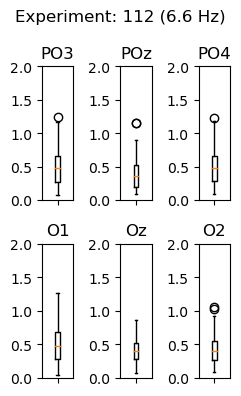
\includegraphics[width=\linewidth]{images/appendix/11266.png}
        \label{fig:11266}
    \end{subfigure}
    \begin{subfigure}{0.25\linewidth}
        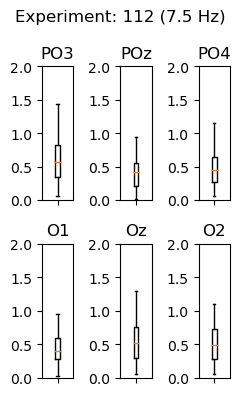
\includegraphics[width=\linewidth]{images/appendix/11275.png}
        \label{fig:11275}
    \end{subfigure}
    \caption{Experiment 2 - Conditions 0, 1, and 2: Boxplots per hemisphere.}
    \label{fig:2-6675}
\end{figure}

\begin{figure}[ht]
    \centering
    \begin{subfigure}{0.3\textwidth}
        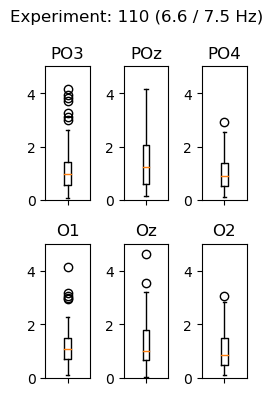
\includegraphics[width=\linewidth]{images/results/1106675.png}
        \label{fig:1106675}
    \end{subfigure}
    \hfill
    \begin{subfigure}{0.3\textwidth}
        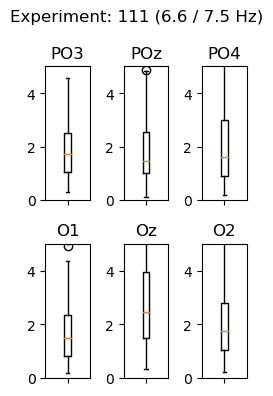
\includegraphics[width=\linewidth]{images/results/1116675.png}
        \label{fig:1116675}
    \end{subfigure}
    \hfill
    \begin{subfigure}{0.3\textwidth}
        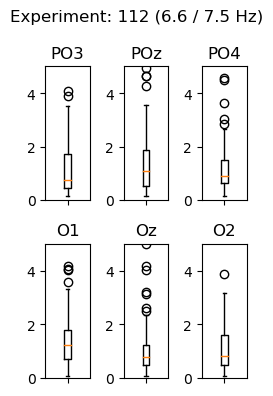
\includegraphics[width=\linewidth]{images/results/1126675.png}
        \label{fig:1126675}
    \end{subfigure}
    \caption{Experiment 2: Boxplot comparisons of amplitude ratios for the different conditions.}
    \label{fig:2-66/75}
\end{figure}


\begin{figure}[ht]
    \centering
    \begin{subfigure}{0.25\linewidth}
        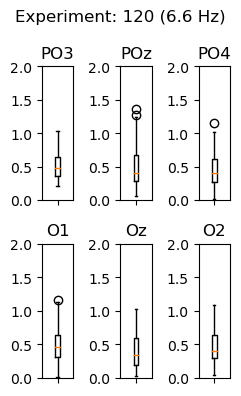
\includegraphics[width=\linewidth]{images/appendix/12066.png}
        \label{fig:12066}
    \end{subfigure}
    \begin{subfigure}{0.25\linewidth}
        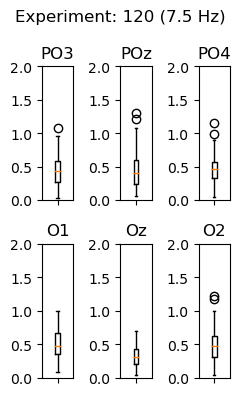
\includegraphics[width=\linewidth]{images/appendix/12075.png}
        \label{fig:12075}
    \end{subfigure}
    \caption{Experiment 3 - Boxplots per hemisphere.}
    \label{fig:3-6675}
\end{figure}


\begin{figure}[ht]
    \centering
    \begin{subfigure}{0.25\linewidth}
        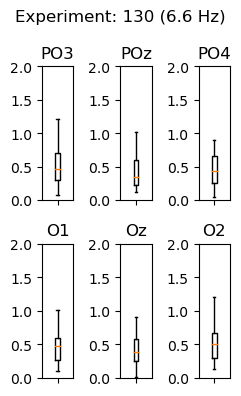
\includegraphics[width=\linewidth]{images/appendix/13066.png}
        \label{fig:13066}
    \end{subfigure}
    \begin{subfigure}{0.25\linewidth}
        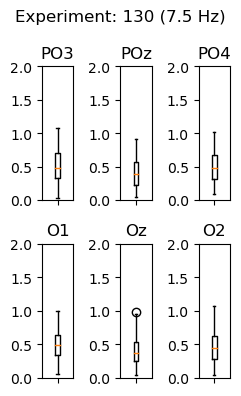
\includegraphics[width=\linewidth]{images/appendix/13075.png}
        \label{fig:13075}
    \end{subfigure}
    
    \begin{subfigure}{0.25\linewidth}
        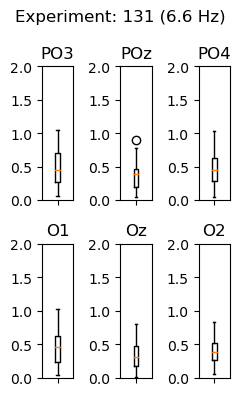
\includegraphics[width=\linewidth]{images/appendix/13166.png}
        \label{fig:13166}
    \end{subfigure}
    \begin{subfigure}{0.25\linewidth}
        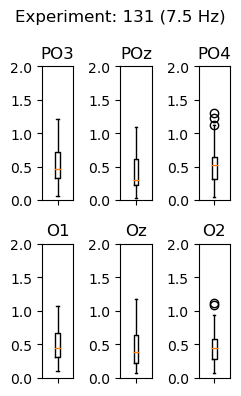
\includegraphics[width=\linewidth]{images/appendix/13175.png}
        \label{fig:13175}
    \end{subfigure}
    \caption{Experiment 4 - Conditions 0, 1, and 2: Boxplots per hemisphere.}
    \label{fig:4-6675}
\end{figure}


\begin{figure}[ht]
    \centering
    \begin{subfigure}{0.25\textwidth}
        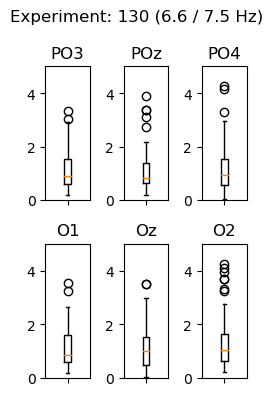
\includegraphics[width=\linewidth]{images/results/1306675.png}
        \label{fig:1306675}
    \end{subfigure}
    \begin{subfigure}{0.25\textwidth}
        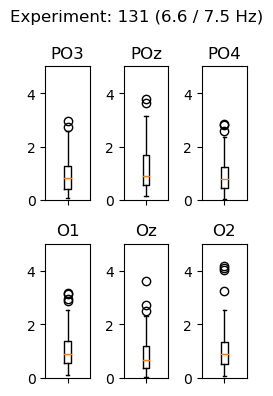
\includegraphics[width=\linewidth]{images/results/1316675.png}
        \label{fig:1316675}
    \end{subfigure}
    \caption{Experiment 4 - Conditions 0 and 1: Boxplots per hemisphere.}
    \label{fig:4-66/75}
\end{figure}


\backmatter
% The bibliography comes after the appendices.
\bibliographystyle{IEEEtran}
\bibliography{chapters/references}

\end{document}
